%\documentclass[referee,sn-mathphys-ay,pdflatex]{sn-jnl}
%\documentclass[sn-mathphys-ay,pdflatex]{sn-jnl}
\documentclass[pdflatex]{sn-jnl}
% Language setting
% Replace `englis' with e.g. `spanish' to change the document language
\usepackage[english]{babel}
\usepackage[utf8]{inputenc} % fuer Umlaute
\usepackage{fontenc}

% Set page size and margins
% Replace `letterpaper' with`a4paper' for UK/EU standard size
%\usepackage[a4paper,top=2cm,bottom=2cm,left=3cm,right=3cm,marginparwidth=1.75cm]{geometry}

%%%% ---- Useful packages

%%% --- Colors
\usepackage[dvipsnames]{xcolor}

%%% --- Figures and Graphics
\usepackage{graphicx}
\usepackage{subcaption}
\usepackage{tikz}

%%% --- Tabulars
\usepackage{booktabs}
\usepackage{multirow} % cells over several rows
\usepackage{tabularx}
%\usepackage{tabularray}
\usepackage{floatrow}
\DeclareFloatFont{tiny}{\tiny}% "scriptsize" is defined by floatrow, "tiny" not
\floatsetup[table]{font=scriptsize} %https://tex.stackexchange.com/a/27100

%%% --- Mathematics
\usepackage{amsmath,amsfonts,amssymb,amsthm,mathtools, mathabx}
\usepackage{bm} % bold mathematics
\usepackage{bbm} % for blackboard 1
\usepackage[linesnumbered,lined,algo2e,figure,boxed]{algorithm2e}
\usepackage[short]{optidef} % for aligning linear programs
%\usepackage{nccmath} % for fleqn environment

%%% --- Other
%\usepackage[colorlinks=true, allcolors=blue]{hyperref}
%\usepackage[hidelinks]{hyperref}
\usepackage[style=authoryear,backend=biber,natbib=true]{biblatex}
%\usepackage{natbib}
%\bibliographystyle{
%\addbibresource{library.bib}
\addbibresource{library-jonas.bib}
\usepackage{csquotes}
\usepackage[shortcuts]{extdash} % For Hyphens in English
%\usepackage{acro}
% \DeclareAcronym{pdf}{short=PDF, long={probability distribution function}}

%%% --- Commenting, Todonotes
\usepackage[colorinlistoftodos,prependcaption]{todonotes}
%\usepackage{comment, soul}
%\newcommand{\ar}{$\rightarrow$}
\presetkeys{todonotes}{backgroundcolor=yellow!30, bordercolor=yellow!50, linecolor=yellow!50, figwidth=\textwidth}{}
%\newcommand{\hl}[1]{\textcolor{Aquamarine}{#1}}

%\usepackage{xargs,ifthen} % Use optional arguements in commands
%\newcommandx{\unsure}[2][1=]{\todo[linecolor=blue,backgroundcolor=blue!25,bordercolor=blue,#1]{#2}}
%\newcommandx{\discuss}[2][1=]{\todo[linecolor=orange,backgroundcolor=orange!25,bordercolor=orange,#1]{#2}}
%\newcommandx{\missing}[2][1=]{\todo[linecolor=red,backgroundcolor=red!25,bordercolor=red,#1]{#2}}
%\newcommandx{\change}[2][1=]{\todo[linecolor=red,backgroundcolor=red!25,bordercolor=red,#1]{#2}}
%\newcommandx{\info}[2][1=]{\todo[linecolor=OliveGreen,backgroundcolor=OliveGreen!25,bordercolor=OliveGreen,#1]{#2}}
%\newcommandx{\improvement}[2][1=]{\todo[linecolor=Plum,backgroundcolor=Plum!25,bordercolor=Plum,#1]{#2}}
%\newcommandx{\done}[2][1=]{\todo[linecolor=gray,backgroundcolor=gray!25,bordercolor=gray,#1]{#2}}
%\newcommandx{\thiswillnotshow}[2][1=]{\todo[disable,#1]{#2}}
%\usepackage{marginnote}
%\let\marginpar\marginnote

%%% --- Acronyms
\usepackage{acro}
\DeclareAcronym{kde}{short=KDE, long=kernel density estimation}
\DeclareAcronym{bca}{short=BCa, long=bias-corrected and accelerated}
\DeclareAcronym{cdf}{short=CDF, long=cumulative distribution function}
\DeclareAcronym{pdf}{short=PDF, long=probability density function}
\DeclareAcronym{nbp}{short=NBP, long=non-invasive blood pressure}
\DeclareAcronym{abp}{short=ABP, long=invasive arterial blood pressure}
\DeclareAcronym{bs}{short=BS, long=Brier score}
\DeclareAcronym{rmse}{short=RMSE, long=root mean square error}
\DeclareAcronym{mae}{short=MAE, long=mean absolute error}
\DeclareAcronym{tadda}{short=TADDA, long=targeted absolute deviation with direction augmentation}
\DeclareAcronym{atc}{short=ATC, long=ability to track changes}
\DeclareAcronym{mnf}{short=MNF, long={measurement, nowcast, or forecast}}


%%%% ---- Own Commands
%%% --- Theorem Settings
\theoremstyle{plain}% Theorem-like structures provided by amsthm.sty
\newtheorem{theorem}{Theorem}
\newtheorem{exa}{Example}
\newtheorem{rem}{Remark}
\newtheorem{proposition}{Proposition}
\newtheorem{lemma}{Lemma}
\newtheorem{corollary}{Corollary}

\theoremstyle{definition}
\newtheorem{definition}{Definition}
\newtheorem{remark}{Remark}
\newtheorem{example}{Example}

%%% --- Math Commands

\DeclarePairedDelimiter{\abs}\lvert\rvert
\DeclareMathOperator{\sign}{sign}
\newcommand{\tmax}{\bar{t}}
\newcommand{\ind}[1]{\mathbbm{1}\{#1\}}
\newcommand{\Prob}[1]{P(#1)}
\newcommand{\cond}{\:\lvert\:}
\newcommand{\card}[1]{\abs{#1}}

\newcommand{\R}{\mathbb{R}}
\newcommand{\N}{\mathbb{N}}
\newcommand{\SBer}{\text{SBer}}

\newcommand{\diffxl}{\mathbf{x}^{\Delta,l}}
\newcommand{\diffyl}{\mathbf{y}^{\Delta,l}}
\newcommand{\diffx}{\mathbf{x}^{\Delta}}
\newcommand{\diffy}{\mathbf{y}^{\Delta}}
\newcommand{\diffxrv}{X^{\Delta}}
\newcommand{\diffyrv}{Y^{\Delta}}
\newcommand{\diffxlt}{\mathbf{x}^{\Delta,l}_t}
\newcommand{\diffylt}{\mathbf{y}^{\Delta,l}_t}
\newcommand{\diffxt}[1][t]{x^{\Delta}_{#1}}
\newcommand{\diffyt}[1][t]{y^{\Delta}_{#1}}

\newcommand{\acc}{\mu}
\newcommand{\accp}{\acc^+}
\newcommand{\accm}{\acc^-}
%\newcommand{\acceps}[1][]{\ifthenelse { \equal {#1} {} }{\acc_{\eps}}{\acc_{#1}}} %https://stackoverflow.com/a/7314951
\newcommand{\acceps}[1][e]{\acc_{#1}} %https://stackoverflow.com/a/7314951
\newcommand{\accpeps}[1][e]{\acceps[#1]^+}
\newcommand{\accmeps}[1][e]{\acceps[#1]^-}
\newcommand{\accl}[1][l]{\mu^{#1}}
\newcommand{\accpl}[1][l]{\acc^{+,#1}}
\newcommand{\accml}[1][l]{\acc^{-,#1}}

\newcommand{\pmax}{\hat{p}} % Notation for the grid resolution in quantiles
\newcommand{\pc}{p^c}

\newcommand{\xcond}{\chi}

%%% --- Other Commands
\renewcommand{\arraystretch}{1.2}

% Ungefähre Wortanzahl des Hauptteils (von Introduction bis Conclusion): oben links auf 'Menu' und dann 'Word Count'
% Ungefähre Aufteilung auf Abschnitte (nicht direkt in Overleaf sichtbar):
% Introduction: 500
% Assessment of ATC: 2225
% Application: 3045
% Discussion and Conclusion: 587

% Abstract: 99



%%% --- ToDo List
%\usepackage{enumitem}
%\newlist{todolist}{itemize}{2}
%\setlist[todolist]{label=$\square$}
%\usepackage{pifont}
%\newcommand{\cmark}{\ding{51}}%
%\newcommand{\xmark}{\ding{55}}%
%\newcommand{\done}{\rlap{$\square$}{\raisebox{2pt}{\large\hspace{1pt}\cmark}}%
%\hspace{-2.5pt}}
%\newcommand{\wontfix}{\rlap{$\square$}{\large\hspace{1pt}\xmark}}

\begin{document}

\title{Assessment of the ability to track changes for measurements, nowcasts, and forecasts}
%\author{Oliver Grothe, Bolin Liu, Jonas Rieger}
\author*[1]{Jonas Rieger}\email{jonas.rieger@kit.edu}
\author[1]{Bolin Liu}
\author[2]{Bernd Saugel}
\author[1]{Oliver Grothe}

\affil[1]{\orgdiv{Institute for Operations Research}, \orgname{Karlsruhe Institute of Technology (KIT)}, \orgaddress{\street{Kaiserstr. 12}, \city{Karlsruhe}, \postcode{76131}, \country{Germany}}}
%TC:ignore
\abstract{ 
In addition to measurements, nowcasts, or forecasts being numerically precise, it is essential [to know] how well they reflect changes in the underlying values.
In this article, we focus on evaluating the ability to predict the correct direction of changes, which we refer to as the ability to track changes (ATC). 
We present visual techniques and quantitative measures to assess this ability and provide extensions for noisy data and estimation uncertainty using bootstrap confidence intervals and exclusion areas.
Worked-through examples illustrate the assessment using the proposed methods: COVID-19-nowcasting, emergency department arrival forecasting, and invasive and non-invasive blood pressure measurements.
}
%TC:endignore
\keywords{}

\maketitle
% \listoftodos



\section{Introduction}\label{sec:atc-introduction}

The appropriate evaluation of \ac{mnf} methods is fundamental for assessing the method's suitability for the task.
If the development of the underlying values is of interest, the ability to predict the correct direction of changes, we call \acf{atc}, is crucial.
Although the three areas differ in the framework and methods used, they share the goal of predicting an unknown value, and thus, similar techniques can be used in the evaluation.

Forecasting methods predict the future based on historical data, patterns, and exogenous factors.
In medicine and healthcare, forecasting is used in various applications, such as population and personal health~\parencite[see, e.g., the review in][]{Soyiri2013}, emergency department demand forecasting~\parencite{Jones2008, Rostami-Tabar2023}, and emergency medical services~\parencite{HaugsboHermansen2021}.
The forecast is computed based on the current value of the quantity of interest and an estimate of the development until the target time.
Methodologically evolved from forecasting~\citep{Browning1989}, nowcasting methods focus on predictions for the present, the immediate future, and the recent past~\citep{Banbura2013, WorldMeteorologicalOrganizationWMO2017}.
Nowcasting methods use high-frequency indicators or preliminary measurements related to the target value and focuses on ongoing predictions due to updating information for the same time~\citep{Castle2017}.
Epidemic nowcasting, for example, can assess the current situation during an ongoing epidemic, considering the main pathogenic, epidemiological, clinical, and socio-behavioral factors~\citep{Wu2021} or correct the daily COVID case numbers for events that have occurred but have not yet been reported~\citep{Gunther2021, Wolffram2023}.
Measurement aims to obtain accurate and reliable data about the current state of a system based on sensors.
Through repeated measurements a system's development is tracked.
When introducing new, cheaper, simpler, or less invasive measurement methods, they are evaluated against current measurement techniques, called the gold standard, by measuring the same quantity in different settings, such as various individuals or environments.

In forecasting and nowcasting, the evaluation is based on accuracy measures such as the \ac{rmse}, probabilistic scoring rules, and calibration measures~\citep{Gneiting2007, Gunther2021, Wolffram2023}.
None of them assesses the method's \ac{atc}.
In a prediction competition on armed conflicts, the assessment of \ac{atc} recently gained attention as \citet{Vesco2022} used the novel \ac{tadda} score with an additive tracking-changes-component for evaluation.
However, the score poses an unintuitive incentive to forecasters and is thus theoretically problematic~\parencite{Bracher2023}.
In measurement agreement analysis, a typical analysis includes the Bland-Altman analysis and a percentage error~\citep{Bland1986}.
The assessment of \ac{atc} is a field of active research in recent years~\citep{Saugel2015, Saugel2018, Hiraishi2021}.

This article focuses on pure assessment of \ac{atc} accompanying traditional scores.
 We formalize \ac{atc} and present different variants of assessment of \ac{atc} measures that consider either noiseless data or data with noise and small non-informative changes (see Section~\ref{sec:aatc}).
We introduce the conditional \ac{atc} plot, a new graphical method for assessing local \ac{atc} behavior, and review bootstrap methods for calculating confidence intervals (see Section~\ref{subsec:aatc-noise} and ~\ref{subsec:aatc-cond-prob}).
We extend the concept of assessment of \ac{atc} to probabilistic predictions in Section~\ref{subsec:aatc-probabilistic}.
The methods are applied to three applications from the abovementioned fields: COVID-19-nowcasting, emergency department arrival forecasting, and blood pressure measurement, and, thus, provide blueprints for future assessments.
The ready-to-use code for the assessment of \ac{atc} from the applications is available on [LINK WILL BE INSERTED].


\section{Assessment of the ability to track changes (ATC)}\label{sec:aatc}

\subsection{Computing changes and notation}\label{subsec:notation}

As noted above, the assessment of \ac{atc} is based on the observed and predicted changes over a time horizon $l$.
The \textit{observed} change is straightforward to compute for all types of \ac{mnf}.
Let $\mathbf{y} = (y_t)_{t=0}^T$ denote the actual values for nowcasting or forecasting, or gold standard measurements up to time $T$.
The sequence of observed changes is then given by the differences of values in $\mathbf{y}$ with horizon $l$, that is,
\begin{equation}\label{eq:diffy}
    \diffylt = (y_{t} - y_{t-l}) \quad \text{for}\ t = l, \dots, T.
\end{equation}

\begin{table}
    \centering
    \scriptsize
    \begin{tabular}{l l}
        \toprule
        Application & Predicted change computation \\
        \midrule
        Measurement & $(x_{t} - x_{t-l})_{t=l}^T $\\
        Nowcasting & $
\diffxl =
\begin{cases}
(x_{t|t} - x_{t-l|t})^T_{t=l}, & \text{if } y_{t-l} \text{ is not known at time } t, \\
(x_{t|t} - y_{t-l})^T_{t=l}, & \text{otherwise}.
\end{cases}
$ \\
        Forecasting & $ \diffxl = (x_{t|t-l} - y_{t-l})^T_{t=l}$\\
        \bottomrule
    \end{tabular}
    \caption[Computation of the predicted change in the different applications.]{Computation of the predicted change in the different applications. For nowcasting and forecasting, $x_{t | \tau}$ refer to values issued at $\tau$ with a target time $t$. For measurement, $x_t$ denotes the test device measurement at time $t$.}
    \label{tab:notation}
\end{table}

The definition of the \textit{predicted} change depends on the context;
Table~\ref{tab:notation} summarizes the notation for \ac{mnf} and the computation of the predicted change.
For nowcasting, let $x_{t | \tau}$ denote the nowcast for time $t$ computed with the knowledge of time $\tau$.
We call $t$ the \textit{target time} and $\tau$ the \textit{issue time}.
The predicted change is computed by
\begin{equation}
  \diffxl =
\begin{cases}
(x_{t|t} - x_{t-l|t})^T_{t=l} & \text{if } y_{t-l} \text{ is not known at time } t, \\
(x_{t|t} - y_{t-l})^T_{t=l} & \text{otherwise}.
\end{cases} \label{eq:diffxl_nowcasting}
\end{equation}
When computing the predicted change of a nowcast for a time $t$, we use the best knowledge available at that time $t$, and the true value might not be known yet.
If the true value $y_{t-l}$ is known at time $t$, the predicted change is computed by the difference between the nowcast and the true value, as $y_{t-l}$ is also known by the nowcaster and incorporated into the nowcast.
Through the computation in Equation~\eqref{eq:diffxl_nowcasting}, the predicted change can be computed with the knowledge of the nowcaster at time $t$.

The notation is similar for forecasting: Let $x_{t | \tau}$ denote the forecast for target time $t$ and issue time $\tau$.
The predicted change is computed by
\begin{equation} \diffxl = (x_{t|t-l} - y_{t-l})^T_{t=l}\label{eq:diffxl_forecasting}
\end{equation}
with the same structure as in the nowcasting case and consistent indices with $\diffyl$.
If the true value $y_{t-l}$ is not known at time $t-l$, a similar modification can be made as in Equation~\eqref{eq:diffxl_nowcasting}.


The distinction between forecast and issue time is unnecessary in measurement analysis, as the measurement is typically available with a very short time lag.
Thus, $x_t$ denotes the test method measurement for time $t$.
The computation
\begin{equation}
  (x_{t} - x_{t-l})_{t=l}^T \label{eq:diffxl_measure}
\end{equation}
yields the change by the test method.
It is computed purely by the test method without the gold standard $y_t$ to analyze whether the gold standard and test method changes are consistent.
Accordingly, $y_{t-l}$ is not used in the computation even if known at time $t$ in contrast to forecasting and nowcasting.

In applications, data are often not available for all time steps, for example, due to technical problems or delays in data transfer (see the examples in Sections~\ref{sec:application-covid} and~\ref{sec:application-eda}).
We refer to time steps for which either \ac{mnf} or true values are unavailable as missing values.
Systematical missing values could lead to a biased assessment, and missing data should be inspected for any underlying patterns.
If the missing values are not systematic, random, and occur scarcely, data pairs with missing values can be excluded from the data to calculate the measures~\parencite[see][Section 1.3]{VanBuuren2018}.
Note that in the case of measurement data, one missing value in the time series leads to two undefined differences in the change series; that is if $x_t$ is missing, $\diffxt$ and $\diffxt[t+l]$ are undefined; if an observation $y_t$ is missing, $\diffyt$ and $\diffyt[t+l]$ are undefined.
The data pair is excluded even if the corresponding nowcast or forecast is available.



\subsection{The four-quadrant plot}\label{subsec:aatc-four-quadrant-plot}

Formally, the assessment of \ac{atc} is the same for \ac{mnf}, given the notation for the respective application of Section~\ref{subsec:notation}.
In the following, we omit the horizon $l$ for ease of notation; $\diffx$ and $\diffy$ refer to $\diffxl$ and $\diffyl$ for a common horizon $l$.
The \ac{atc} is maximal if all predicted change directions are correct; that is, the sign of all elements of $\diffx$ and $\diffy$ coincide.
Consequently, when assessing the \ac{atc}, we examine the statistical consistency of $\sign(\diffx)$ and $\sign(\diffy)$.
A simple yet insightful method is the four-quadrant plot~\citep[see, e.g., ][]{Perrino1998, Saugel2015}.
In a four-quadrant plot, the occured changes and the predicted changes are plotted together, that is, $(\diffyt, \diffxt)$ for $t = l, \dots, T$.
Thus, the x-axis of a four-quadrant plot shows the true value differences, whereas the y-axis displays the prediction data differences.
Points in the green upper right and lower left quadrants reflect a correct change direction for the respective time step, whereas points in the remaining red quadrants show incorrectly predicted changes.
Figure~\ref{fig:aatc_basic_4q} displays a basic four-quadrant plot and Figure~\ref{fig:aatc_basic_4q_sample} shows a four-quadrant graph for simulated data with $T=1461$, for example, four years of daily data.

The four-quadrant plot can be extended by including information on the time index in the point color to reveal effects over time.
In Figure~\ref{fig:aatc_basic_4q_sample_color}, the point colors turn from blue to green for higher time indices $t$, that is, more recent values; $(\diffyt[l], \diffxt[l])$ is blue and turns green until $(\diffyt[T], \diffxt[T])$.
However, four-quadrant plots become crowded for larger datasets, and sequential information on the differences is complex to assess thoroughly.

The four-quadrant plot is intuitive to interpret, and the magnitude and direction of change are shown simultaneously.
Other visualization techniques, such as polar plots, lack the four-quadrant plot's clarity and intuition without adding more information on the \ac{atc}~\citep{Saugel2015}.

\begin{figure}
\centering
\begin{subfigure}[t]{.24\textwidth}
\includegraphics{plots/illustrative_examples/4Q_without_excl}
\caption{Basic four-quadrant plot.} \label{fig:aatc_basic_4q}
\end{subfigure}\hspace{0.01\textwidth}%
\begin{subfigure}[t]{.24\textwidth}
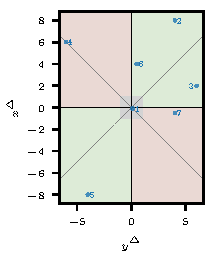
\includegraphics{plots/illustrative_examples/4q_excl_box}
\caption{Four-quadrant plot with rectangular exclusion area. Point 1 is excluded.}\label{fig:aatc_basic_4q_excl_box}
\end{subfigure}\hspace{0.01\textwidth}%
\begin{subfigure}[t]{.24\textwidth}
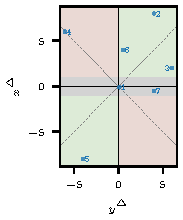
\includegraphics{plots/illustrative_examples/4q_excl_axis}
\caption{Four-quadrant plot with horizontal exclusion area. Points 1 and 7 are excluded.} \label{fig:aatc_basic_4q_excl_axis}
\end{subfigure}\hspace{0.01\textwidth}%
\begin{subfigure}[t]{.24\textwidth}
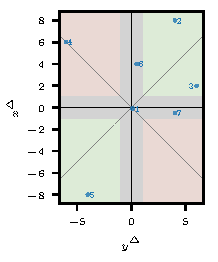
\includegraphics{plots/illustrative_examples/4q_excl_cross}
\caption{Four-quadrant plot with cross-shaped exclusion area. Points 1, 6 and 7 are excluded.}\label{fig:aatc_basic_4q_excl_cross}
\end{subfigure}%
\caption{Illustrations of the four-quadrant plot with sample points and with and without exclusion areas. The rectangular exclusion area in Figure~\ref{fig:aatc_basic_4q_excl_box} excludes only points where both components are likely to be noise-driven, while the exclusion areas in Figures~\ref{fig:aatc_basic_4q_excl_axis} and~\ref{fig:aatc_basic_4q_excl_cross} excludes points where at least one component is noise-driven. }
\label{fig:aatc_4q}
\end{figure}

\subsection{ATC ratio and other measures}\label{subsec:atc-measures}

Analyzing the number of points in the green versus red quadrants is a standard approach in the \ac{atc} assessment of measurement data~\citep{Critchley2010, Saugel2015}.
With that, we estimate the probability of a correctly predicted change direction, $P(\diffxrv \diffyrv > 0)$, where $\diffyrv$ and $\diffxrv$ denote random variables for future incremental changes.
Since $z_1 z_2 > 0$ imposes the same condition as $\sign(z_1) = \sign(z_2)$ ($z_1, z_2 \in \R \setminus \{ 0 \}$), the standard estimator for $P(\diffxrv \diffyrv > 0)$ is
\begin{equation}
    \acc (\diffx, \diffy) \coloneqq \frac{\sum_{t \in \mathcal{T}} \ind{\diffxt \diffyt > 0}}{\card{T}}.\label{eq:acc}
\end{equation}
Here, the numerator counts the number of same-sign-changes, while the denominator is the number of considered pairs $(\diffyt, \diffxt)$.
Thus, $\acc$ is the proportion of concordant changes on all changes.
We refer to this estimator as the \textit{ATC ratio} of the prediction and set $\mathcal{T} = \{l, \dots, T\}$.
Visually, the measure computes the fraction of points in the upper right or lower left quadrant.
Similar evaluations are used in other scientific areas, for example, with contingency tables in dichotomous forecasting or with confusion matrices in classification analysis~\citetext{see, e.g., the introductions in \citealt{James2021}, Ch. 4, and \citealp{Jolliffe2012}, Ch. 3}.
Many other measures can be adapted from those fields to deepen the analysis.
Two simple measures that focus on a positive or negative predicted change are the positive and negative \ac{atc} ratios $\accp$ and $\accm$, respectively.
They are defined as
\begin{align}
    \accp (\diffx, \diffy) &\coloneqq \frac{\sum_{t \in \mathcal{T}} \ind{\diffxt \diffyt > 0} \ind{\diffxt > 0}}{\sum_{t \in \mathcal{T}} \ind{\diffxt > 0}},\ \text{and} \label{eq:accp}\\
    \accm (\diffx, \diffy) &\coloneqq \frac{\sum_{t \in \mathcal{T}} \ind{\diffxt \diffyt > 0} \ind{\diffxt < 0}}{\sum_{t \in \mathcal{T}} \ind{\diffxt < 0}}.\label{eq:accm}
\end{align}
They estimate the probability of a correct prediction of the direction of change, given that the predicted direction is positive or negative, that is, $P(\diffxrv \diffyrv > 0 | \diffxrv > 0)$ and $P(\diffxrv \diffyrv > 0 | \diffxrv < 0)$.

Rolling estimates of the above measures detect changes in performance over time and can give a sharper estimate of the current \ac{atc}.
For the ATC ratio, a rolling estimate with a backward-looking window of length $w$ at time $t$ is given by
\begin{equation*}
    \acc_{t; w} (\diffx, \diffy) \coloneqq \frac{\sum_{t^\star = t-w + 1}^{t} \ind{\diffxt[t^\star] \diffyt[t^\star] > 0}}{w}.\label{eq:acc_rolling}
\end{equation*}
Backward-looking windows estimate the ATC ratio at a time $t$ considering the $w$ time steps before time $t$.
The window length $w$ controls the smoothing of the estimate; a larger $w$ gives smoother results, while a small $w$ focuses on local variations.
Plotting the rolling estimates for $t = w-1, \dots, T$ yields an estimate of the ATC ratio over time.
Figure~\ref{fig:atc_ratio_time_series} depicts a rolling window estimate of the ATC ratio for the simulated data of Figures~\ref{fig:aatc_basic_4q_sample} and~\ref{fig:aatc_basic_4q_sample_color}.
While colored four-quadrant plots, as in Figure~\ref{fig:aatc_basic_4q_sample_color}, illustrate ongoing overall drifts in the \ac{atc}, seasonal aspects are only revealed in rolling window estimates.


\begin{figure}
    \centering
    \begin{subfigure}[t]{.24\textwidth}
\includegraphics{plots/illustrative_examples/4Q_sample_without_time}
\caption{Four-quadrant plot with simulated data.}\label{fig:aatc_basic_4q_sample}
\end{subfigure}\hspace{0.01\textwidth}
\begin{subfigure}[t]{.24\textwidth}
\includegraphics{plots/illustrative_examples/4Q_sample_with_time}
\caption{The same data is colored according to the time index $t$, the greener, the later.}\label{fig:aatc_basic_4q_sample_color}
\end{subfigure}\hspace{0.01\textwidth}
\begin{subfigure}[t]{.48\textwidth}
    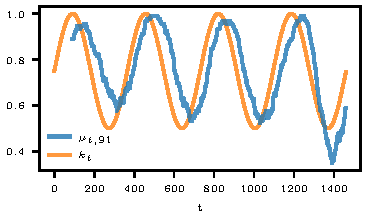
\includegraphics{plots/illustrative_examples/trending_ratio_time_series}
    \caption{Rolling estimate of the \ac{atc} ratio over time with window length 91. }\label{fig:atc_ratio_time_series}
    \end{subfigure}%
    \caption[Visualizations of the four-quadrant plot for data with a time-varying ATC ratio.]{Visualizations for data with a time-varying ATC ratio. We defer information on the data generation process to the appendix (see \ref{subsec:app-ATC-data-generation}). The ATC ratio for the entire data set is $\mu = 0.7577$. The strong seasonality of the ATC ratio becomes visible in Figure~\ref{fig:atc_ratio_time_series}. The green curve $k_t$ shows the theoretical probability that $\diffxt$ has the same sign as $\diffyt$ for each time step. The rolling estimates are shifted to the right compared to $k_t$ as the windows look backward. Thus, the yearly course of the ATC ratio can be detected.
The ATC ratio has a pronounced sinus-shaped seasonality with a peak after a quarter of a year and a low point after three quarters.
}
\end{figure}

\subsection{Accounting for noise and non-informative small changes and bootstrapping confidence intervals}\label{subsec:aatc-noise}

The above measures can be extended to account for information on the point's location within the quadrant.
For example, points close to the zero point may have less explanatory power or may be less reliable than points far away from zero on one of the diagonals.
Suppose noise or non-systematic effects are present in the true values or predictions.
In that case, noise can drive a point's assignment to a quadrant instead of a systematic \ac{atc}.
This is more likely for points with at least one small coordinate.

Using an exclusion area around the zero point, as further defined below, is a straightforward and highly interpretable extension of the measures of Section~\ref{subsec:atc-measures} accounting for such effects~\citep[see, e.g.,][]{Saugel2015, Critchley2010}.
Points within that area are omitted in the calculation of the measures.
In particular, the \ac{mnf} are likely to have a noise component; thus, $\diffx$ should be subject to an exclusion area.
The measures of Equations~\eqref{eq:acc},~\eqref{eq:accp} and~\eqref{eq:accm} without points in the exclusion area $E$ are
\begin{align}
    \acceps (\diffx, \diffy, E) &\coloneqq \frac{\sum_{t \in \mathcal{T}} \ind{\diffx \diffy > 0} \ind{(\diffyt, \diffxt) \notin E}}{\sum_{t \in \mathcal{T}} \ind{(\diffyt, \diffxt) \notin E}},\label{eq:acceps}\\
    \accpeps (\diffx, \diffy, E) &\coloneqq \frac{\sum_{t \in \mathcal{T}} \ind{\diffxt \diffyt > 0} \ind{\diffxt > 0, (\diffyt, \diffxt) \notin E}}{\sum_{t \in \mathcal{T}} \ind{\diffxt > 0, (\diffyt, \diffxt) \notin E}}, \ \text{and} \label{eq:accpeps}\\
    \accmeps (\diffx, \diffy, E) &\coloneqq \frac{\sum_{t \in \mathcal{T}} \ind{\diffxt \diffyt > 0} \ind{\diffxt < 0, (\diffyt, \diffxt) \notin E}}{\sum_{t \in \mathcal{T}} \ind{\diffxt < 0, (\diffyt, \diffxt) \notin E}}. \label{eq:accmeps}
\end{align}
The measures are then estimators for the probability of predicting the correct direction, given that the point's location is not driven by noise or non-informative changes.

The estimators accept various shapes of the exclusion area (see Figure~\ref{fig:aatc_4q}).
A rectangular exclusion area, $E = \{(y, x) \in \R^2: (-\varepsilon_x \leq x \leq \varepsilon_x) \land (-\varepsilon_y \leq y \leq \varepsilon_y) \}$ for $\varepsilon_x, \varepsilon_y > 0$, leaves out points that are small in both components.
%Points are included if the true value or prediction is unlikely to be noise-driven.
%In the example graph in Figure~\ref{fig:aatc_basic_4q_excl_box}, only point 1 is excluded.
An exclusion area along one axis, for example, $E = \{(y, x) \in \R^2: (-\varepsilon_x \leq x \leq \varepsilon_x)\}$ for $\varepsilon_x > 0$, removes points in which one of the components could change sign by a small amount of noise.
%At least for \ac{mnf}, small amounts of noise are inevitable.
A cross-shaped exclusion area, $E = \{(y, x) \in \R^2: (-\varepsilon_x \leq x \leq \varepsilon_x) \lor (-\varepsilon_y \leq y \leq \varepsilon_y) \}$ for $\varepsilon_x, \varepsilon_y > 0$, along both axes accounts for the sign reversal in both components.
%A point is only included if no component is likely to be driven by noise.
%For the latter two methods, points 1 and 7 in Figure~\ref{fig:aatc_basic_4q_excl_axis} or 1, 6, and 7 are excluded in Figure~\ref{fig:aatc_basic_4q_excl_cross}, respectively.

In most applications, the shape and size of the exclusion area can be chosen based on domain knowledge or expert opinions.
The size determination can also be based on a proportion of the total variance or the total range of the data; for example, the 10\% smallest absolute values in each component determine the exclusion area size.
A third approach is to visualize the \ac{atc} ratio for different sizes of $E$ and thus inspect the effects of the exclusion area size on the estimates.
For examples of such plots, see Section~\ref{sec:application-covid}.

Confidence intervals can account for the estimation uncertainty of the measures above.
Bootstrap confidence intervals are based on resampling and not on parametric assumptions as classical confidence intervals are~\parencite[for introductions see][]{Hesterberg2011, Bittmann2021}.
Many new samples are drawn with replacement from the dataset, and the statistic of interest is computed for each sample, yielding an estimate for the distribution of the statistic of interest.
Based on the derived \enquote{new} samples of the statistic, the confidence intervals can be derived through different bootstrapping methods.
We use the \ac{bca} approach for bootstrapping in the following, as it holds the confidence level for small and large samples and has a moderate computation time (see the simulation study in Appendix~\ref{subsec:appendix-aatc-bootstrap}).


\subsection{The conditional ATC plot}\label{subsec:aatc-cond-prob}

The estimators described above give information on the probabilities $P(\diffxrv \diffyrv > 0 | \diffxrv \diffyrv \notin E)$, $P(\diffxrv \diffyrv > 0 | \diffxrv > 0, \diffxrv \diffyrv \notin E)$ and $P(\diffxrv \diffyrv > 0 | \diffxrv < 0, \diffxrv \diffyrv \notin E)$.
A still finer analysis might be gained by considering the conditional distribution $P(\diffxrv \diffyrv > 0 | \diffxrv = \xcond)$ to assess the \ac{atc} of a prediction for a specific change $\diffxrv = \xcond$ of the \ac{mnf}.
Thereby, $P(\diffxrv \diffyrv > 0 | \diffxrv = \xcond)$ denotes the probability of a correct direction given a predicted change of $\xcond$.
Thus, if a change of $\xcond$ is observed in practice, one can directly assess its credibility.
A multivariate \acf{kde} facilitates a continuous estimation of $P(\diffxrv \diffyrv > 0 | \diffxrv = \xcond)$ by estimating the components $f_{\diffxrv, \diffyrv}$ and $f_{\diffxrv}$ of
\begin{align*}
P(\diffxrv \diffyrv > 0 | \diffxrv = \xcond) = \begin{cases}
                                              \int_{-\infty}^0 \frac{f_{\diffxrv, \diffyrv}(\xcond, y)}{f_{\diffxrv}(\xcond)} \ \textrm{d} \: y & \text{if } \xcond < 0, \\
                                              \int_{0}^{\infty} \frac{f_{\diffxrv, \diffyrv}(\xcond, y)}{f_{\diffxrv}(\xcond)} \ \textrm{d} \: y & \text{if } \xcond > 0, \\
\end{cases}
\end{align*}
for $\xcond \neq 0$ through a \ac{kde}.
\textcite{Gramacki2018} provides a comprehensive introduction to multivariate \ac{kde}, and implementations are available in many programming languages, for example, in the \verb|statsmodels| in Python~\parencite{Seabold2010}.
The \ac{kde} yields estimates for $P(\diffxrv \diffyrv > 0 | \diffxrv = \xcond)$ for all values of $\xcond \in \R$.
Multivariate \ac{kde} takes a kernel and bandwidth selector as modeling parameters.
We advise using a Gaussian kernel and the cross-validation maximum likelihood as bandwidth selector (see Appendix~\ref{subsec:appendix-kde}).

Assessing $P(\diffxrv \diffyrv > 0 | \diffxrv = \xcond)$ graphically by drawing $P(\diffxrv \diffyrv > 0 | \diffxrv = \xcond)$ against $\xcond$ eases the simultaneous evaluation of various $\xcond$.
Furthermore, the graph facilitates the comparison of various methods in a single graph, and asymmetries of $P(\diffxrv \diffyrv > 0 | \diffx = \xcond)$ with respect to $\xcond$ in the \ac{atc} can be detected.
We refer to the plot as a \textit{conditional ATC plot}.



\subsection{Probabilistic evaluation}\label{subsec:aatc-probabilistic}

In nowcasting and forecasting, probabilistic predictions have become more prevalent in recent years (see Sections~\ref{sec:application-covid} and~\ref{sec:application-eda}).
In this section, we develop \ac{atc} assessments for probabilistic measurements and nowcasts.
Probabilistic predictions issue a probability distribution for the quantity of interest based on their available information and, thus, include a point estimate and information on the prediction uncertainty and quantiles simultaneously.
Probabilistic predictions thus also contain a probability of a positive or negative change.
For \ac{atc} assessment, we compare the predicted probability of positive change, denoted by $p_t$, with the occurrence of positive changes.

Probabilistic predictions can be a \ac{cdf}, \ac{pdf}, or quantiles.
The \ac{cdf} is the most general and can be used to derive the others, given that they exist.
Let us first assume that the prediction is a \ac{cdf}, and that $y_{t-l}$ is known at time $t$ (see Table~\ref{tab:notation}).
Appendix~\ref{subsec:app-probabilistic-atc-evaluation} extends the analysis to quantile predictions or unknown true values.

Let for a forecast $F_{t | t-l} (x)$ denote the predicted \ac{cdf} for target time $t$ and issue time $t - l$, where the index is analogous to the point notation of Section~\ref{subsec:notation}.
The \ac{cdf} $F_{t | t-l} (x)$ specifies the forecasted probability that the quantity of interest is at most $x$.
A positive change occurs for any value at $t$ larger than the true value $y_{t-l}$ and the \ac{cdf} $F_{t | t-l} (y_{t-l})$ yields the predicted probability of any value at most $y_{t-l}$, and, thus, a negative change.
Accordingly, the forecasted probability of a positive change is
\begin{equation*}
    p_t = 1 - F_{t | t-l} (y_{t-l})\quad t = l, \dots, T.
\end{equation*}
The computation differs slightly for nowcasts, that is,
\begin{equation*}
    p_t = 1 - F_{t | t} (y_{t-l})\quad t = l, \dots, T,
\end{equation*}
with analogous derivations as above.
Let $z_t$ denote the indicator that the observed change at time $t$ is positive, that is,
\begin{equation*}
    z_t = \ind{\diffyt > 0} \quad t = l, \dots, T.
\end{equation*}
The predictive power of $\mathbf{p} = (p_t)_{t=l}^{T}$ for $\mathbf{z} = (z_t)_{t=l}^{T}$ can be assessed using probabilistic dichotomous forecast evaluation methods.
Dichotomous forecasts predict a binary outcome, such as a positive or negative change, and are evaluated numerically using scoring rules or visually through reliability diagrams.

The \ac{bs} is a widely used scoring rule for dichotomous probabilistic forecasts~\citep{Brier1950}.
In our context, it is
\begin{equation*}
    BS (\mathbf{p}, \mathbf{z}) = \frac{1}{T-l+1} \sum_{t=l}^{T} (p_t - z_t)^2.
\end{equation*}
Lower values indicate the considered method's higher probabilistic \ac{atc}.
The \ac{bs} assesses the calibration and sharpness of the forecast and the observation simultaneously~\citep{Ranjan2010, Mitchell2011}.
Calibration refers to the statistical consistency of forecasts and observations; that is, the event occurs with the issued probability and is considered the more fundamental quality~\citep{Gneiting2007}.
Sharpness refers to the spread of the forecast; probabilities close to zero and one are preferable as they convey a higher certainty.

Graphical methods are a standard tool for evaluating the calibration of probabilistic forecasts in detail.
In dichotomous forecasting, the reliability diagram is frequently used~\citep{Ranjan2010}.
The reliability diagram plots the observed frequency of the positive outcome against the (binned) predicted probability.
For example, it shows the proportion of observed increases, given that the predicted probability of increase was approximately $0.7$.
Ideally, the predicted probability equals the observed frequency, and the reliability diagram is a 45-degree line.
Local deviations from the 45-degree line indicate a miscalibration for specific forecast probabilities.
Thus, the reliability visualizes the local and overall calibration simultaneously.
For an example of a reliability diagram, see Section~\ref{sec:application-eda}.


\section{Application to measurement, nowcasting, and forecasting data} \label{sec:application}

\subsection{Covid nowcasting} \label{sec:application-covid}

In Germany, the seven-day hospitalization rate was established as a central steering measure for COVID-19 in November 2021, and the imposition of severe public restrictions was based on it~\citep{RobertKochInstitute2021}.
However, the publication of the definite rate was subject to severe delays and revisions in two sources.
The first source is technical delays in the reporting process, for example, due to different authorities passing the data to the RKI~\citep{RobertKochInstitute2024}.
The second, more systematic source is the structure of the seven-day hospitalization rate, allocating all Covid-related hospitalization to the date of the first positive test~\parencite[for a detailed description, see][]{Wolffram2023}.
Nevertheless, as the seven-day hospitalization rate was considered a central indicator of the pandemic's development, various organizations and institutions issued nowcasts.
The COVID19-Nowcasting-Hub collected various nowcasts in a predefined setup, including the seven-day hospitalization rate's predictive mean, median, and other quantiles~\citep{ChairOfEconometricsAndStatisticsAtKarlsruheInstituteOfTechnology2024}.
For information on the model design, nowcast tasks, and the data submission guidelines, we refer to~\citet{Wolffram2023}.
Table~\ref{tab:app-covid-models} matches the abbreviations here to the respective names in the COVID19-Nowcasting-Hub.
In addition to those nowcasts, \citet{Wolffram2023} construct two ensemble methods using the ensembles' mean or median.
We denote them by ENS-MEAN and ENS-MED.
In line with the initial study design, we consider the period from November 22, 2021, to April 29, 2022, as the evaluation period.
We use the data from February 8, 2024, for the true values and focus on nowcasts for all inhabitants of Germany.
Figure~\ref{fig:app-covid-true-nowcast} in Appendix~\ref{sec:appendix-application-covid} displays the true and nowcast data for the evaluation period.
The time comprises the fourth wave's end in December 2021 and nearly the entire fifth wave of the pandemic in Germany, lasting until May 28, 2022~\citep{Tolksdorf2022}.

To assess the impact of taken measures and the direction of the curve, the knowledge of whether hospitalization rates rise or fall is essential.
Thus, the \ac{atc} assessment is particularly relevant for the nowcasts of the seven-day hospitalization rate.
If hospitalization rates rise, measures should be tightened, while falling rates might allow for loosening measures.
Asymmetries are especially relevant for assessing whether some models are better at recognizing a fall than a rise or vice versa.

\subsubsection*{Results}

\begin{table}
    \centering
    \begin{tabular}{llllr}
\toprule
 & rmse & mae & mse & count \\
model &  &  &  &  \\
\midrule
ILM-prop & :,.f & :,.f & :,.f & 530 \\
RIVM-KEW & :,.f & :,.f & :,.f & 817 \\
NowcastHub-MeanEnsemble & :,.f & :,.f & :,.f & 610 \\
NowcastHub-MedianEnsemble & :,.f & :,.f & :,.f & 610 \\
LMU_StaBLab-GAM_nowcast & :,.f & :,.f & :,.f & 574 \\
RKI-weekly_report & :,.f & :,.f & :,.f & 334 \\
KIT-simple_nowcast & :,.f & :,.f & :,.f & 861 \\
SZ-hosp_nowcast & :,.f & :,.f & :,.f & 535 \\
SU-hier_bayes & :,.f & :,.f & :,.f & 423 \\
Epiforecasts-independent & :,.f & :,.f & :,.f & 275 \\
\bottomrule
\end{tabular}

    \caption[Point evaluation measures for the issued mean of the different models in Covid nowcasting.]{Point evaluation measures for the issued mean of the different models in Covid nowcasting. \enquote{RMSE} and \enquote{MAE} are accuracy measures, while \enquote{Count} lists the number of non-missing values. The RMSE orders the models. The evaluation period comprises 159 days and only few nowcasts are missing~\citep[for explanations of the missing values, see][Tables A2, A3, and A4]{Wolffram2023}. Note that the high values for the EPI model could be driven by an exceptionally far-off value at the end of the evaluation period (see Figure~\ref{fig:app-covid-true-nowcast}).}
    \label{tab:app-covid-rmse}
\end{table}

Table~\ref{tab:app-covid-rmse} summarizes the non-\ac{atc}-aware point evaluation measures for the issued mean of the different models.
The best-performing models in terms of RMSE and MAE are the ILM and RKI models.
The ensemble methods ENS-MED and ENS-MEAN perform worse than the best models regarding the mean location.
The performance of the models is diverse, with more than twice as high RMSE values for the worst models compared to the best models.

In the following, we apply the \ac{atc} assessment for the short-term horizons one and medium-term horizons seven and 14 days.
The horizons seven and 14 reflect a typical period until new policy changes are taken.
We start by providing background information on the marginal distributions of the actual value and nowcast changes for the different horizons in Table~\ref{tab:app-covid-marginals} in Appendix~\ref{sec:appendix-application-covid} such as standard deviation and quantiles of the nowcasts and true values.
The variability and general level of changes grow with the horizon: The standard deviation increases from roughly 300 for horizon one to 1,200 for horizon seven and 2,000 for horizon 14 days.
Similarly, the 10\%-quantile of changes, the basis for the exclusion area size, increases.
The exclusion area is rectangular; a point falls within it if both $\diffy$ and $\diffx$ are below the respective 10\%-quantile of the absolute changes.
Thus, points are still included in the \ac{atc} assessment if they are large in one dimension but not in the other, thus ensuring that substantial changes in, for example, $\diffy$ are to be recognized by the nowcast and vice versa.

\begin{table}
    \centering
    \tiny
    \begin{tabular}{l p{0.11\textwidth} p{0.11\textwidth} p{0.11\textwidth} p{0.11\textwidth} p{0.11\textwidth} p{0.11\textwidth}}
\toprule
 & $\mu^{7}$ & $\mu^{+, 7}$ & $\mu^{-, 7}$ & $\mu^{7}_{q_{0.1}}$ & $\mu^{+, 7}_{q_{0.1}}$ & $\mu^{-, 7}_{q_{0.1}}$ \\
\midrule
EPI & {0.77\newline(0.71, 0.82)} & {0.67\newline(0.59, 0.76)} & {0.87\newline(0.79, 0.92)} & {0.78\newline(0.72, 0.83)} & {0.68\newline(0.59, 0.75)} & {0.88\newline(0.80, 0.93)} \\
ILM & {0.85\newline(0.80, 0.90)} & {0.73\newline(0.64, 0.80)} & {0.99\newline(0.94, 1.00)} & {0.85\newline(0.80, 0.90)} & {0.74\newline(0.65, 0.81)} & {0.99\newline(0.94, 1.00)} \\
KIT & {0.74\newline(0.68, 0.80)} & {0.64\newline(0.55, 0.72)} & {0.87\newline(0.80, 0.93)} & {0.75\newline(0.69, 0.80)} & {0.64\newline(0.55, 0.72)} & {0.88\newline(0.81, 0.94)} \\
LMU & {0.80\newline(0.74, 0.85)} & {0.70\newline(0.62, 0.77)} & {0.91\newline(0.84, 0.95)} & {0.81\newline(0.75, 0.86)} & {0.72\newline(0.63, 0.79)} & {0.92\newline(0.85, 0.96)} \\
ENS-MEAN & {0.82\newline(0.76, 0.86)} & {0.71\newline(0.63, 0.78)} & {0.94\newline(0.89, 0.97)} & {0.82\newline(0.76, 0.87)} & {0.71\newline(0.63, 0.78)} & {0.96\newline(0.90, 0.99)} \\
ENS-MED & {0.82\newline(0.77, 0.86)} & {0.70\newline(0.61, 0.78)} & {0.96\newline(0.90, 0.99)} & {0.83\newline(0.77, 0.87)} & {0.72\newline(0.64, 0.79)} & {0.96\newline(0.90, 0.99)} \\
RIVM & {0.83\newline(0.77, 0.87)} & {0.74\newline(0.65, 0.81)} & {0.92\newline(0.86, 0.96)} & {0.83\newline(0.78, 0.88)} & {0.74\newline(0.65, 0.81)} & {0.93\newline(0.87, 0.97)} \\
RKI & {0.72\newline(0.65, 0.77)} & {0.60\newline(0.51, 0.67)} & {0.98\newline(0.92, 1.00)} & {0.73\newline(0.66, 0.78)} & {0.61\newline(0.53, 0.68)} & {0.98\newline(0.92, 1.00)} \\
SU & {0.81\newline(0.75, 0.86)} & {0.71\newline(0.62, 0.79)} & {0.92\newline(0.85, 0.96)} & {0.81\newline(0.75, 0.85)} & {0.71\newline(0.63, 0.79)} & {0.92\newline(0.85, 0.96)} \\
SZ & {0.78\newline(0.72, 0.83)} & {0.67\newline(0.58, 0.75)} & {0.91\newline(0.84, 0.96)} & {0.78\newline(0.72, 0.83)} & {0.67\newline(0.58, 0.75)} & {0.92\newline(0.85, 0.97)} \\
\bottomrule
\end{tabular}

    \caption[The ATC ratios for Covid nowcasting.]{The \ac{atc} ratio $\accl[7]$, positive \ac{atc} ratio $\accpl[7]$, and negative \ac{atc} ratio $\accml[7]$ for the models without and with exclusion areas for the horizon seven days in Covid nowcasting. The exclusion areas are rectangles centered on the zero points with a width and height of twice the 10\%-quantile of the absolute values of nowcast and true values. The subscript $q_{0.1}$ denotes the measures with exclusion area. }
    \label{tab:app-covid-atc-ratios-lag-7}
\end{table}

Table~\ref{tab:app-covid-atc-ratios-lag-7} lists the \ac{atc} ratios for all models without and with exclusion areas for the horizon of seven days.
The \ac{atc} ratios without exclusion area range from 0.72 to 0.85 for the horizon of seven days.
The negative \ac{atc} ratios are higher than the positive \ac{atc} ratios for all models.
The confidence intervals for the positive and negative \ac{atc} ratios do not overlap for all models, indicating that the \ac{atc} ratios are indeed different.
The 10\%-quantile exclusion areas have, at most, an influence of 0.03 on the ratios.
The model with the highest \ac{atc} ratio is the ILM model, and the model with the lowest is the RKI model.
The confidence intervals between all models without and with exclusion areas overlap.
The positive \ac{atc} ratio implies a similar ranking of the models than the overall \ac{atc}, while the negative ratio provides a different ranking, for example, for the RKI model.
For the horizons of one and 14 days, we refer to Table~\ref{tab:app-covid-atc-ratios-lag-1-14} in Appendix~\ref{sec:appendix-application-covid}.

\begin{figure}
    \centering
%    \includegraphics{}
    \begin{subfigure}[t]{.48\textwidth}
    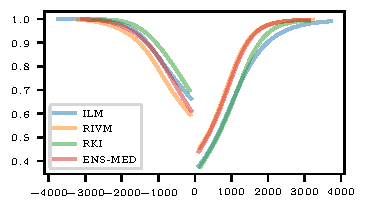
\includegraphics{plots/covid_nowcast/40_cond_prob_lag_7}
    \caption{Conditional ATC plot.}\label{fig:app-covid-cond-prob-7}
    \end{subfigure}\hfill
    \begin{subfigure}[t]{.48\textwidth}
    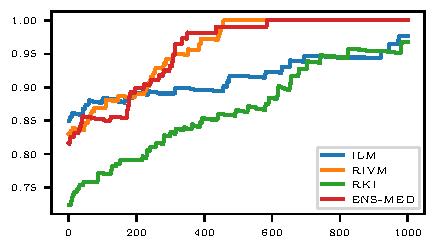
\includegraphics{plots/covid_nowcast/40_acc_eps_lag_7}
    \caption{ATC ratio over exclusion area size in $\diffx$.}\label{fig:app-covid-atc-ratio-7}
    \end{subfigure}
    \caption[Conditional ATC plot and ATC ratio over exclusion area for the Covid nowcasts.]{Conditional \ac{atc} plot and \ac{atc} ratio over exclusion area for the nowcasts of the seven-day hospitalization rate ILM, RKI, RIVM, and ENS-MED for the horizon seven days in Covid nowcasting.}
    \label{fig:app-covid-cond-prob-atc-ratio-7}
\end{figure}

Figure~\ref{fig:app-covid-cond-prob-atc-ratio-7} shows the conditional \ac{atc} plots and the \ac{atc} ratio over the exclusion area for the horizon seven days; the respective plots for the horizons one day and 14 days are shown in Figure~\ref{fig:app-covid-cond-prob-atc-ratio-1-14}.
Here, only the best models in point evaluation measures, ILM, RKI, RIVM, and ENS-MED, are shown to keep the plots easily readable.
If RKI or ILM issues a fall in the hospitalization rate, the probability of a fall is higher than if RIVM or ENS-MED issues a fall.
The opposite is the case for a nowcasted hospitalization rate increase, and the difference between the models' performance is more prominent than for a fall.
Similar observations can be made for the horizon of 14 days in Figure~\ref{fig:app-covid-cond-prob-14}.
For a horizon of one day, the models' conditional ATC difference is less pronounced (see Figure~\ref{fig:app-covid-cond-prob-1}).
The RKI model is still less conclusive when issuing an increase in the hospitalization rate, while RIVM is most informative in that case.
The curves cross for an issued fall, with ENS-MED being on top for issued falls above 250.

The \ac{atc} ratios for various exclusion areas are shown in Figure~\ref{fig:app-covid-atc-ratio-7}.
The \ac{atc} ratio generally increases with larger exclusion areas.
While the RIVM and ENS-MED \ac{atc} ratios evolve similarly, the RKI and ILM \ac{atc} ratios get closer.
For the horizon of one day, the RKI \ac{atc} ratio decreases with increasing exclusion area size while the other models rise (see Figure~\ref{fig:app-covid-atc-ratio-1}).
For the horizon of 14 days, all \ac{atc} ratio curves increase with the exclusion area size (see Figure~\ref{fig:app-covid-atc-ratio-14}).

Figure~\ref{fig:app-covid-prob} shows the \acf{bs} and reliability diagrams for the same subset of models, the ILM, RKI, RIVM, and ENS-MED.
The probabilities of increase for the different models are computed using the nowcast quantiles.
For each horizon $l$, $10,000$ samples of the forecast date $t$ and the forecast date $t-l$ based on the nowcasts of issue date $t$ are generated, and the proportion of positive changes is computed (see Appendix~\ref{subsec:app-probabilistic-atc-evaluation}).
Remember that a low \ac{bs} and a reliability diagram along the diagonal are signs of a high \ac{atc}.
The \ac{bs} is the lowest for the RIVM model for a one-day-horizon, while the ENS-MED model has the best \ac{bs} for the horizon of seven and 14 days.
The RKI model yields the highest \ac{bs} for all horizons.
Note that the \ac{bs} is 0.25 for random guessing; thus, all models perform better than random guessing.
The reliability diagrams show that the models are not well calibrated for the horizon of one day.
While for predicted probabilities below 0.5, the observed ratio of increases is smaller, it is higher than predicted for probabilities above 0.5.
Figure~\ref{fig:app-covid-prob-hist} shows the observed predicted increase probabilities for all horizons.
For the horizons of seven and 14 days, the nowcasters issue only a few moderate probabilities, and most probabilities are near zero and one.

\begin{figure}
    \begin{subfigure}{0.48\textwidth}
        \centering
        \tiny
        \begin{tabular}{llll}
\toprule
 & 1 d & 7 d & 14 d \\
\midrule
ILM & 0.1783 & 0.1269 & 0.1119 \\
RIVM & 0.1606 & 0.1136 & 0.1274 \\
RKI & 0.1893 & 0.2200 & 0.1712 \\
ENS-MED & 0.1812 & 0.1096 & 0.1066 \\
\bottomrule
\end{tabular}

    \caption{BS for the different models and horizons.}\label{fig:app-covid-prob-brier}
    \end{subfigure}\hspace{0.01\textwidth}%
    \begin{subfigure}[t]{0.48\textwidth}
    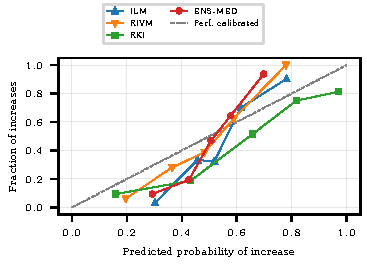
\includegraphics{plots/covid_nowcast/60_reliability_diagram_lag_1}
    \caption{Reliability diagram for horizon one day.}\label{fig:app-covid-prob-rel-1}
    \end{subfigure}\hspace{0.01\textwidth}%
    \caption[Brier Scores and reliability diagrams for the Covid nowcasting models ILM, RKI, RIVM, and ENS-MED.]{\aclp{bs} and reliability diagrams for the Covid nowcasting models ILM, RKI, RIVM, and ENS-MED.
    The reliability diagram bins are chosen according to the empirical quantiles of the predicted probabilities.
    In the computation of BS and reliability diagram, missing values are excluded.
    The reliability diagram for the horizon seven and 14 days is in the appendix (see Figure~\ref{fig:app-covid-rel}).}
    \label{fig:app-covid-prob}
\end{figure}





\subsubsection*{Discussion}

For all horizons, the influence of the exclusion area on the 10\%-quantile level is negligible.
For example, the \ac{atc} ratio changes at most by 0.03 for the EPI model with $\accml[14]$.
The exclusion areas are thus not crucial for the \ac{atc} assessment in the case of the nowcasts of the seven-day hospitalization rate.
The lower bound of confidence intervals is at least 0.68 for all models, indicating that they perform better than random guessing the trend.

\ac{atc} assessment evaluates the models differently from point evaluation measures.
RKI is among the best in point evaluation measures but performs worse in \ac{atc} assessment.
The assessment of asymmetry in the conditional \ac{atc} plots is crucial for interpreting the \ac{atc} ratios, with the RKI model being the most prominent example.

Figure~\ref{fig:app-covid-atc-ratio-7} shows that larger exclusion areas increase the \ac{atc} ratio, indicating that the predicted direction is more accurate for large predicted changes.

The probabilistic \ac{atc} assessment shows that the models are better than random guessing.
The reliability diagram cannot provide information if specific probabilities are issued scarcely.
Thus, the reliability diagrams for the horizons of seven and 14 days do not contain information on moderate probabilities.
The \ac{bs} values, however, work well for those examples and provide a good measure for the \ac{atc} of the models.

A more extensive data size would be beneficial for assessing the models' performance.
For the evaluation period of 159 days, the \ac{atc} ratio confidence intervals overlap; thus, no conclusions can be drawn from the \ac{atc} assessment comparing the models.

\subsection{Forecasting emergency department arrivals}\label{sec:application-eda}

In a second example, we consider forecasting the number of arrivals in a large emergency department per hour with data and models by \citet{Rostami-Tabar2023}.
Every 12 hours, the models issue hourly forecasts for the next 48 hours.

\citet{Rostami-Tabar2023} publish means and probabilistic quantile forecasts for various models and input data.
We use the published mean as a point forecast for the \ac{atc} assessment and evaluate the probabilistic \ac{atc} based on the quantile forecasts subsequently.
Considering only the forecasts of at least 36 hours ahead, we restrict the evaluation period to March 2, 2018, at noon, to February 28, 2019, at 23:00, comprising 8,724 hours.

In this setup, \ac{atc} assessment is a simple and intuitive way to assess the models' performance.
The \ac{atc} perspective is easy for the management to understand and implement, as simple comparisons of the expected workload to a recent shift can be made.
If, for example, the staff was near capacity during the last shift and an increase in the number of arrivals is expected, management can take measures to adjust the workload.

The number of arrivals has a strong weekly and daily pattern.
Thus, we consider the horizons of 72 hours, the last already observed shift of the same hour of day, and seven days, the previous shift of the same hour and day, in \ac{atc} assessment.

\subsubsection*{Results}

Table~\ref{tab:app-eda-point-evaluation} lists the point evaluation measures and the count of available forecasts.
The best-performing models regarding RMSE and MAE are the NBI-2 and Poisson-2 models.
More than 8,600 forecasts are available for all models, with changes in the number due to missing values on four afternoons in 2018.

\begin{table}
\centering
\begin{tabular}{l r r r}
\toprule
Model & RMSE & MAE & Count \\
\midrule
NBI-2 & 8.883 & 3.200 & 8688 \\
Poisson-2 & 8.884 & 3.200 & 8688 \\
Poisson-1 & 9.164 & 3.238 & 8688 \\
Benchmark-2 & 9.246 & 3.236 & 8688 \\
Ttr-2 & 9.394 & 3.266 & 8688 \\
NOtr-1 & 9.413 & 3.276 & 8688 \\
NOtr-2 & 9.413 & 3.276 & 8688 \\
Poisson-2-I & 9.458 & 3.276 & 8688 \\
Benchmark-1 & 10.065 & 3.331 & 8688 \\
GBM-2 & 11.663 & 3.542 & 8688 \\
tbats & 12.905 & 3.912 & 8724 \\
Prophet & 13.078 & 3.877 & 8724 \\
qreg-1 & 13.337 & 3.758 & 8688 \\
Regression-Poisson & 21.162 & 4.818 & 8724 \\
ADAM-iETSX & 28.000 & 5.561 & 8724 \\
ETS & 29.358 & 5.742 & 8724 \\
\bottomrule
\end{tabular}

\caption[Point evaluation measures for the emergency department arrival forecasting models.]{Point evaluation measures for the emergency department arrival forecasting models. The smaller count for some models stems from missing forecasts scattered throughout the evaluation period. Note that the reported values for the RMSE differ from those in \citet{Rostami-Tabar2023} due to differences in the evaluation period.}\label{tab:app-eda-point-evaluation}
\end{table}

We start by analyzing the marginal distributions for the predicted and observed changes for the three- and seven-day horizons in Table~\ref{tab:app-eda-marginals}, again.
The computed difference aligns with Section~\ref{subsec:notation}, that is, the difference between the forecasted mean and true value of three and seven days before, as the actual value is available when issuing the forecast.
The positive change fraction varies between 0.39 and 0.63 for the horizon of three days and between 0.37 and 0.63 for the horizon of seven days.
The variability of changes decreases for the larger horizon for most models; only for the ETS model does it increase.
The 10\%-quantile of the changes is between zero and one for all models and horizons.
Thus, we use an exclusion area of size 1.
The resulting fraction of included values in the computation is also listed in Table~\ref{tab:app-eda-marginals} and is at least 79\% of the values.

\begin{table}
    \centering
    \tiny
    \begin{tabular}{lllllllll}
\toprule
 & (1), l=3 & $\sigma_{x^{\Delta, 3}}$ & $q_{0.1} (x^{\Delta, 3})$ & (2), l=3 & (1), l=7 & $\sigma_{x^{\Delta, 7}}$ & $q_{0.1} (x^{\Delta, 7})$ & (2), l=7 \\
\midrule
ADAM-iETSX & 0.57 & 7.76 & 0.83 & 0.88 & 0.57 & 7.49 & 0.78 & 0.87 \\
Benchmark-1 & 0.45 & 5.05 & 0.50 & 0.80 & 0.44 & 4.43 & 0.47 & 0.78 \\
Benchmark-2 & 0.51 & 5.11 & 0.52 & 0.80 & 0.50 & 4.29 & 0.45 & 0.78 \\
ETS & 0.58 & 7.49 & 0.78 & 0.87 & 0.58 & 7.68 & 0.84 & 0.88 \\
GBM-2 & 0.39 & 4.93 & 0.51 & 0.80 & 0.37 & 4.61 & 0.49 & 0.79 \\
NBI-2 & 0.53 & 5.04 & 0.52 & 0.81 & 0.53 & 4.41 & 0.48 & 0.79 \\
NOtr-1 & 0.52 & 5.03 & 0.51 & 0.81 & 0.51 & 4.41 & 0.49 & 0.79 \\
NOtr-2 & 0.52 & 5.03 & 0.51 & 0.81 & 0.51 & 4.41 & 0.49 & 0.79 \\
Poisson-1 & 0.53 & 5.04 & 0.51 & 0.81 & 0.52 & 4.38 & 0.48 & 0.79 \\
Poisson-2 & 0.53 & 5.05 & 0.52 & 0.80 & 0.53 & 4.42 & 0.48 & 0.78 \\
Poisson-2-I & 0.51 & 5.03 & 0.51 & 0.81 & 0.50 & 4.42 & 0.49 & 0.79 \\
Prophet & 0.62 & 5.27 & 1.00 & 0.91 & 0.62 & 5.15 & 1.00 & 0.91 \\
Regression-Poisson & 0.51 & 6.65 & 0.67 & 0.85 & 0.51 & 6.49 & 0.67 & 0.85 \\
Ttr-2 & 0.51 & 5.03 & 0.50 & 0.81 & 0.50 & 4.41 & 0.49 & 0.79 \\
qreg-1 & 0.39 & 5.01 & 0.49 & 0.81 & 0.39 & 4.84 & 0.51 & 0.80 \\
tbats & 0.63 & 5.35 & 1.00 & 0.92 & 0.63 & 5.04 & 1.00 & 0.92 \\
True & 0.54 & 6.61 & 1.00 & 0.93 & 0.55 & 5.90 & 1.00 & 0.92 \\
\bottomrule
\end{tabular}

    \caption[Marginal analysis of the forecast and true changes in emergency department arrival forecasting.]{Marginal analysis of the forecast and true changes in emergency department arrival forecasting. The column (1) shows the fraction of values greater than zero for horizon $l$, $\sigma_{x^{\Delta, l}}$ the standard deviation, and $q_{0.1} (x^{\Delta, l})$ the 10\% quantile of the changes' absolute values. Column (2) shows the fraction of values not in the exclusion area of size one.}
    \label{tab:app-eda-marginals}
\end{table}

Table~\ref{tab:app-eda-atc-ratios} lists the \ac{atc} ratios for all models for three and seven-day horizons.
The \ac{atc} ratios range from 0.68 to 0.84 for a horizon of three days and from 0.68 to 0.82 for seven days.
The negative and positive \ac{atc} ratios differ for all models and horizons.
For some models, for example, the GBM-2 model, the positive \ac{atc} ratio is higher than the negative \ac{atc} ratio, and for some models, for example, the tbats model, vice versa.
The confidence interval width is at most 0.02 for the \ac{atc} ratios and at most 0.03 for the positive and negative \ac{atc} ratios.
The models GBM-2, qreg-1, and Benchmark-1 have the highest positive \ac{atc} ratio for the three and seven-day horizon, while Poisson-2 and NBI-2 have the highest negative \ac{atc} ratio.

Figure~\ref{fig:app-eda-cond-prob} shows the conditional \ac{atc} plots for the models Benchmark-1, GBM-2, NBI-2, Poisson-2, and qreg-1 for the horizons three and seven days and thus inspects the local \ac{atc} of the models with highest positive and negative \ac{atc} ratio.
The conditional \ac{atc} plots show similar courses for the two horizons, though the curves are shifted downwards for the horizon of seven days.
The model's relative \ac{atc} evolves consistently for the two horizons, with the NBI-2 and Poisson-2 models being indistinguishable.
The GBM-2 model outperforms the qreg-1 model for all predicted changes.
The models NBI-2 and Poisson-2 have the highest \ac{atc} for all negative predicted changes and the lowest for all positive predicted changes.
Benchmark-1 lies between the other models for all predicted changes.

Figure~\ref{fig:app-eda-prob} visualizes the probabilistic \ac{atc} assessment for the same subset of models.
The \acfp{bs} are shown in Figure~\ref{fig:app-eda-prob-brier}, and the reliability diagrams for the horizons three and seven days in Figures~\ref{fig:app-eda-prob-rel-3} and~\ref{fig:app-eda-prob-rel-7}.
The \acp{bs} are smallest for NBI-2 and Poisson-2 for both horizons, while the \acp{bs} for the other models are larger and differ more.
The qreg-1 model has both horizons' highest \ac{bs}.
The reliability diagrams of GBM-2 and NBI-2 are also close and show a too-small fraction of increases for the predicted probability overall.
For the other models, the reliability diagrams show a fraction of increases that are too large for the corresponding predicted probability.

\begin{table}
    \centering
    \tiny
    \begin{tabularx}{\textwidth}{X p{0.11\textwidth} p{0.11\textwidth} p{0.11\textwidth} p{0.11\textwidth} p{0.11\textwidth} p{0.11\textwidth}}
\toprule
 & $\mu^{3}$ & $\mu^{+, 3}$ & $\mu^{-, 3}$ & $\mu^{7}$ & $\mu^{+, 7}$ & $\mu^{-, 7}$ \\
\midrule
ADAM-iETSX & {0.70\newline(0.69, 0.71)} & {0.68\newline(0.67, 0.69)} & {0.72\newline(0.71, 0.73)} & {0.68\newline(0.67, 0.69)} & {0.67\newline(0.66, 0.69)} & {0.69\newline(0.67, 0.70)} \\
Benchmark-1 & {0.83\newline(0.82, 0.84)} & {0.86\newline(0.85, 0.87)} & {0.81\newline(0.79, 0.82)} & {0.81\newline(0.80, 0.82)} & {0.86\newline(0.85, 0.87)} & {0.78\newline(0.76, 0.79)} \\
Benchmark-2 & {0.84\newline(0.83, 0.84)} & {0.83\newline(0.82, 0.85)} & {0.84\newline(0.83, 0.85)} & {0.82\newline(0.81, 0.83)} & {0.83\newline(0.82, 0.84)} & {0.80\newline(0.79, 0.82)} \\
ETS & {0.68\newline(0.67, 0.69)} & {0.66\newline(0.65, 0.67)} & {0.70\newline(0.69, 0.72)} & {0.67\newline(0.66, 0.68)} & {0.66\newline(0.64, 0.67)} & {0.68\newline(0.66, 0.69)} \\
GBM-2 & {0.82\newline(0.81, 0.82)} & {0.90\newline(0.89, 0.91)} & {0.77\newline(0.76, 0.78)} & {0.78\newline(0.77, 0.79)} & {0.88\newline(0.87, 0.90)} & {0.73\newline(0.72, 0.74)} \\
NBI-2 & {0.84\newline(0.83, 0.85)} & {0.83\newline(0.82, 0.84)} & {0.85\newline(0.84, 0.86)} & {0.82\newline(0.81, 0.83)} & {0.82\newline(0.81, 0.83)} & {0.82\newline(0.81, 0.83)} \\
NOtr-1 & {0.83\newline(0.83, 0.84)} & {0.83\newline(0.82, 0.84)} & {0.84\newline(0.82, 0.85)} & {0.81\newline(0.80, 0.82)} & {0.82\newline(0.81, 0.83)} & {0.80\newline(0.79, 0.81)} \\
NOtr-2 & {0.83\newline(0.83, 0.84)} & {0.83\newline(0.82, 0.84)} & {0.84\newline(0.82, 0.85)} & {0.81\newline(0.80, 0.82)} & {0.82\newline(0.81, 0.83)} & {0.80\newline(0.79, 0.81)} \\
Poisson-1 & {0.84\newline(0.83, 0.84)} & {0.82\newline(0.81, 0.83)} & {0.85\newline(0.84, 0.86)} & {0.82\newline(0.81, 0.82)} & {0.82\newline(0.81, 0.83)} & {0.81\newline(0.80, 0.82)} \\
Poisson-2 & {0.84\newline(0.83, 0.85)} & {0.83\newline(0.82, 0.84)} & {0.85\newline(0.84, 0.86)} & {0.82\newline(0.81, 0.82)} & {0.82\newline(0.81, 0.83)} & {0.82\newline(0.80, 0.83)} \\
Poisson-2-I & {0.83\newline(0.83, 0.84)} & {0.84\newline(0.83, 0.85)} & {0.83\newline(0.82, 0.84)} & {0.81\newline(0.80, 0.82)} & {0.83\newline(0.81, 0.84)} & {0.80\newline(0.79, 0.81)} \\
Prophet & {0.75\newline(0.74, 0.76)} & {0.72\newline(0.71, 0.73)} & {0.79\newline(0.77, 0.80)} & {0.74\newline(0.73, 0.74)} & {0.72\newline(0.70, 0.73)} & {0.76\newline(0.75, 0.77)} \\
Regression-Poisson & {0.72\newline(0.71, 0.73)} & {0.73\newline(0.71, 0.74)} & {0.72\newline(0.70, 0.73)} & {0.70\newline(0.69, 0.71)} & {0.71\newline(0.70, 0.73)} & {0.69\newline(0.67, 0.70)} \\
Ttr-2 & {0.84\newline(0.83, 0.84)} & {0.84\newline(0.83, 0.85)} & {0.83\newline(0.82, 0.85)} & {0.81\newline(0.80, 0.82)} & {0.83\newline(0.82, 0.84)} & {0.80\newline(0.79, 0.81)} \\
qreg-1 & {0.80\newline(0.79, 0.80)} & {0.88\newline(0.87, 0.89)} & {0.75\newline(0.74, 0.76)} & {0.77\newline(0.76, 0.78)} & {0.86\newline(0.85, 0.88)} & {0.71\newline(0.70, 0.72)} \\
tbats & {0.75\newline(0.74, 0.76)} & {0.72\newline(0.71, 0.73)} & {0.80\newline(0.78, 0.81)} & {0.73\newline(0.72, 0.74)} & {0.71\newline(0.69, 0.72)} & {0.76\newline(0.74, 0.77)} \\
\bottomrule
\end{tabularx}

    \caption[ATC ratios for the emergency department arrival forecasts.]{\Ac{atc} ratio $\acc$, positive \ac{atc} ratio $\accp$, and negative \ac{atc} ratio $\accm$ for the models with the exclusion of zero-containing points for the horizons 72 hours and seven days in emergency department arrival forecasting.}
    \label{tab:app-eda-atc-ratios}
\end{table}

\begin{figure}
    \centering
    \begin{subfigure}[t]{0.48\textwidth}
    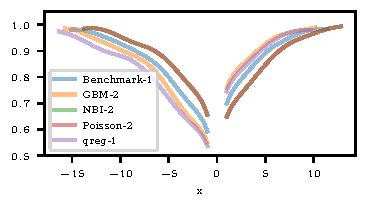
\includegraphics{plots/ed_arrival/50_Cond_Prob_lag_3}
    \caption{Horizon three days}
    \end{subfigure}\hfill
    \begin{subfigure}[t]{0.48\textwidth}
    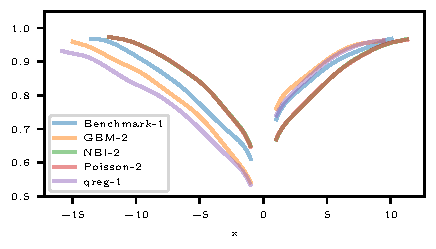
\includegraphics{plots/ed_arrival/50_Cond_Prob_lag_7}
    \caption{Horizon seven days}
    \end{subfigure}
    \caption[Conditional ATC plots for the horizons three and seven days and the models with the best positive or negative \ac{atc} in emergency department arrival forecasting.]{Conditional \ac{atc} plots for the horizons three and seven days and the models with the best positive or negative \ac{atc} in emergency department arrival forecasting. The plots of NBI-2 and Poisson-2 are indistinguishable.}
    \label{fig:app-eda-cond-prob}
\end{figure}

\begin{figure}
    \begin{subfigure}{0.32\textwidth}
    \tiny
    \begin{tabular}{lll}
\toprule
 & 3 d & 7 d \\
\midrule
Benchmark-1 & 0.1586 & 0.1761 \\
GBM-2 & 0.1590 & 0.1759 \\
NBI-2 & 0.1549 & 0.1717 \\
Poisson-2 & 0.1549 & 0.1714 \\
qreg-1 & 0.1679 & 0.1843 \\
\bottomrule
\end{tabular}

    \caption{BS for the different models and horizons.}\label{fig:app-eda-prob-brier}
    \end{subfigure}\hspace{0.01\textwidth}%
    \begin{subfigure}[t]{0.32\textwidth}
    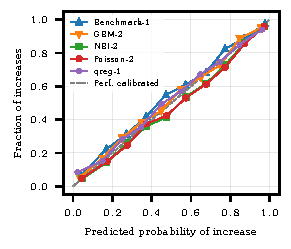
\includegraphics{plots/ed_arrival/60_reliability_diagram_lag_3}
    \caption{Reliability diagram for horizon three days.}\label{fig:app-eda-prob-rel-3}
    \end{subfigure}\hspace{0.01\textwidth}%
    \begin{subfigure}[t]{0.32\textwidth}
    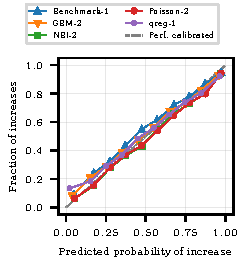
\includegraphics{plots/ed_arrival/60_reliability_diagram_lag_7}
    \caption{Reliability diagram for horizon seven days.}\label{fig:app-eda-prob-rel-7}
    \end{subfigure}
    \caption[Probabilistic \ac{atc} assessment in emergency department arrival forecasting.]{Probabilistic \ac{atc} assessment for the models Benchmark-1, GBM-2, NBI-2, Poisson-2, and qreg-1 for the horizons three and seven days in emergency department arrival forecasting. The \acl{bs} in Figure~\ref{fig:app-eda-prob-brier} evaluates the calibration and sharpness of the probabilistic \ac{atc} simultaneously, while the two plots on the right assess solely the calibration, that is, whether the predicted probability of increase occurs empirically. Probabilistic \ac{atc} by the \ac{bs} is best for the models NBI-2 and Poisson-2 for both lags.}
    \label{fig:app-eda-prob}
\end{figure}

\subsubsection*{Discussion}

The \ac{atc} is consistent for the two horizons, with the models' relative \ac{atc} evolving similarly for the two horizons.
The models' \ac{atc} is generally higher for the smaller horizon, but the changes are minor, and confidence intervals overlap.

The positive and negative \ac{atc} ratios differ for all models.
While some models, such as GBM-2 and qreg-1, have the highest positive \ac{atc} ratio, others, such as Poisson-2 and NBI-2, have the highest negative \ac{atc} ratio.
Thus, the uncertainty of the model's predicted change has to be assessed differently based on the direction.

The probabilistic \ac{atc} assessment results endorse the point \ac{atc} assessment and assign the best scores to NBI-2 and Poisson-2.
The reliability diagrams show that they underestimate the fraction of increases slightly.

Overall, the example provides performance assessments that are different from standard point evaluation measures and thus provide further insights into the strengths and weaknesses of the models.
While the models with the lowest RMSE, NBI-2, and Poisson-2, also have a high \ac{atc}, three models with below-average point evaluation measures, Benchmark-1, GBM-2, and qreg-1, have a high positive \ac{atc}.


\subsection{Invasive and non-invasive blood pressure monitoring} \label{sec:application_measurement}

In the last briefer example, we consider the \ac{atc} assessment of measurement data.
The data is from the MIMIC-III database, including various numerical measurement data, such as heart rate, blood pressure, and oxygen saturation, on patients in critical care units of the Beth Israel Deaconess Medical Center in Boston (Massachusetts, USA, \cite{Johnson2016}, \citealp{Moody2017}; available through \citealp{Goldberger2000}).
We focus on \acf{abp} and \acf{nbp} measurements.
While non-invasive blood pressure measurement methods are relatively gentle, they are less accurate than invasive methods~\citet[see][]{Saugel2014}.
For critical patients, changes in blood pressure can be crucial for the treatment.
Thus, \ac{atc} assessment can be performed in addition to standard accuracy analysis~\citep[see, for example, ][]{Mostafa2020}.
Thus, we assess the \ac{atc} of the non-invasive blood pressure measurements compared to the invasive blood pressure measurements.
The database contains 64,168 numerical data records, comprising all numerical measurements for one patient.
The measured signals vary in length, frequency, and type of measurement.
Thus, only a subset of the data contains measurements of \ac{abp} and \ac{nbp} simultaneously.
2,548 include at least one measurement of systolic \ac{abp} and \ac{nbp} and 1,327 include at least one measurement of systolic \ac{abp} and \ac{nbp} at the same time; for the mean \ac{abp} and \ac{nbp}, the numbers are 2,605 and 1,516, respectively.
We consider the horizons of one minute, five minutes, and 15 minutes for the \ac{atc} assessment, as those are typical intervals of NBP measurements.

\subsubsection*{Results}

Again, we exclude the smallest 10\% of absolute changes in \ac{atc} assessment.
The resulting four-quadrant plots of the mean and systolic blood pressure measurements for the different horizons are shown in Figure~\ref{fig:app-mimic-4q}.
The number of points in the four-quadrant plot is smaller due to the restriction to data records with measurements of mean or systolic \ac{abp} and \ac{nbp} simultaneously for two consecutive times with the specified horizons.
Thus, we use the \ac{nbp} measurements as the test method and the \ac{abp} measurements as the gold standard.
For the systolic measurements, 290, 332, and 442 points are available for the horizons of one, five, and 15 minutes; for the mean measurements, 406, 430, and 542.

The \ac{atc} ratios, including confidence intervals for the different horizons, are listed in Table~\ref{tab:app-mimic-atc-ratios}.
The confidence intervals have lower bounds of 0.5 or slightly above for the measurements with a horizon of one minute.
For larger horizons, the \ac{atc} ratio increases.
The difference between positive and negative \ac{atc} ratios is small for all types and horizons, with overlapping confidence intervals.

Figure~\ref{fig:app-mimic-cond-prob} shows the conditional \ac{atc} plots for the different horizons and the systolic and mean blood pressure measurements.
It becomes apparent that the systolic measurements have a higher \ac{atc} than the mean measurements, except for small negative predicted changes.

\begin{figure}
    \centering
    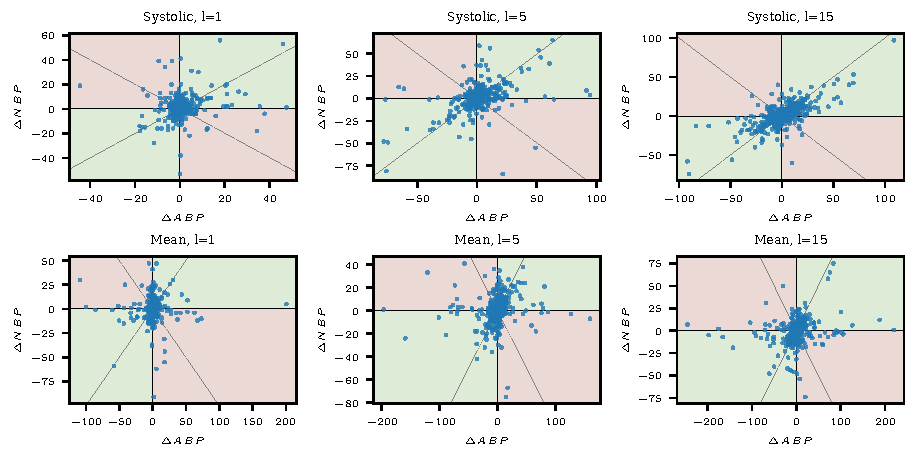
\includegraphics{plots/mimic/plot_4q}
    \caption[Four-quadrant plots for the different horizons and the systolic and mean blood pressure measurements. ]{Four-quadrant plots for the different horizons $l$ and the systolic and mean blood pressure measurements. The upper row contains systolic measurements, and the lower row contains mean measurements. The columns contain the horizons one, five, and 15 minutes.}
    \label{fig:app-mimic-4q}
\end{figure}

\begin{table}
    \centering
    \begin{tabular}{l l p{0.2\textwidth} p{0.2\textwidth} p{0.2\textwidth}}
\toprule
Type & $l$ & $\mu^{l}$ & $\mu^{+, l}$ & $\mu^{-, l}$ \\
\midrule
Systolic & 1 & {0.55 (0.50, 0.60)} & {0.59 (0.52, 0.65)} & {0.58 (0.50, 0.66)} \\
Systolic & 5 & {0.63 (0.59, 0.68)} & {0.70 (0.64, 0.75)} & {0.62 (0.56, 0.69)} \\
Systolic & 15 & {0.69 (0.65, 0.73)} & {0.72 (0.66, 0.76)} & {0.74 (0.69, 0.79)} \\
Mean & 1 & {0.55 (0.51, 0.59)} & {0.62 (0.56, 0.68)} & {0.56 (0.50, 0.62)} \\
Mean & 5 & {0.59 (0.55, 0.64)} & {0.65 (0.59, 0.71)} & {0.62 (0.56, 0.68)} \\
Mean & 15 & {0.62 (0.58, 0.65)} & {0.65 (0.60, 0.70)} & {0.66 (0.61, 0.71)} \\
\bottomrule
\end{tabular}

    \caption[ATC ratios for the different horizons $l$ and the systolic and mean blood pressure measurements.]{\Ac{atc} ratios for the different horizons $l$ and the systolic and mean blood pressure measurements.}
    \label{tab:app-mimic-atc-ratios}
\end{table}

\begin{figure}
    \centering
    \begin{subfigure}[t]{.32\textwidth}
        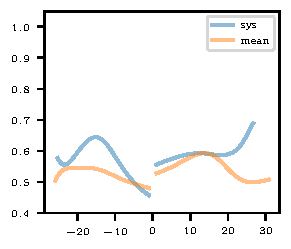
\includegraphics{plots/mimic/cond_prob_diff_nbp_abp_lag1}
        \caption{Horizon one minute.}
    \end{subfigure}\hspace{0.01\textwidth}
    \begin{subfigure}[t]{.32\textwidth}
        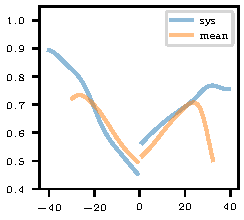
\includegraphics{plots/mimic/cond_prob_diff_nbp_abp_lag5}
        \caption{Horizon five minutes.}
    \end{subfigure}\hspace{0.01\textwidth}
    \begin{subfigure}[t]{.32\textwidth}
        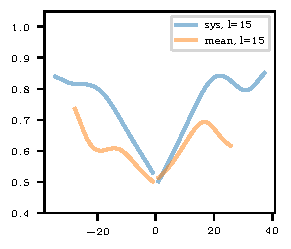
\includegraphics{plots/mimic/cond_prob_diff_nbp_abp_lag15}
        \caption{Horizon 15 minutes.}
    \end{subfigure}\hspace{0.01\textwidth}
    \caption{Conditional ATC plot for the systolic and mean blood pressure measurements and the horizons one, five, and 15 minutes. }
    \label{fig:app-mimic-cond-prob}
\end{figure}




\subsubsection*{Discussion}

The four-quadrant plots contain a considerable number of extreme points.
Whether these points are due to measurement errors or extreme values is not distinguishable.
Some authors argue to exclude the measurements below the 10\%-quantile of the absolute changes and the points above the 90\%-quantile~\citep[see][]{Critchley2010}.
We do not follow this approach here, as the extreme values are not necessarily measurement errors and could be particularly relevant.

The difference between positive and negative \ac{atc} ratios is small in this example.
The positive and negative \ac{atc} ratios have overlapping confidence intervals, the conditional \ac{atc} plots do not contain prominent deviations in the course, and the four-quadrant plots do not display asymmetries.

The bootstrap confidence intervals are wide.
The width is around 0.1 for the \ac{atc} ratio, while it gets up to 0.16 for the negative \ac{atc} ratio for systolic measurement and the horizon of one minute.
Thus, the confidence intervals cover 0.5 for systolic measurement and the horizon of one minute, and the equality to random guessing cannot be excluded.



\section{Discussion and conclusion}\label{sec:atc-conclusion}

In this paper, we examine various methods to assess the \acf{atc} for \acf{mnf}, that is, whether it predicts the correct direction of changes.
While the computation of predicted change varies between the application areas measurement, nowcasting, and forecasting, the predict the correct direction of changes assessment using the computed predicted and observed change is similar.
The \ac{atc} assessment can accompany other evaluation techniques, such as measures of deviation or probabilistic scoring rules.

Four-quadrant plots facilitate the visual inspection of the \ac{atc} for a \ac{mnf} (see Section~\ref{subsec:aatc-four-quadrant-plot}).
The \ac{atc} ratio, the ratio of change directions predicted correctly over the total number of changes, numerically evaluates \ac{atc}.
Visually, it is the proportion of concordant points in a four-quadrant plot (see Section~\ref{subsec:atc-measures}).
The positive and negative \ac{atc} ratios analyze the \ac{atc} ratio given whether the predicted change is positive or negative, respectively.
Thus, they quantify the credibility of the respective predictions.
The applications of Section~\ref{sec:application_measurement} show that models, in general, indeed have different positive and negative \ac{atc} and that they add valuable information to the \ac{atc} ratio.
In the applications, the bootstrap confidence intervals of Section~\ref{subsec:atc-measures} are used to quantify the estimation uncertainty of the \ac{atc} measures.
The width of the confidence intervals is around 0.1 for around 100 samples, while it is around 0.01 for 8000 samples.
For models with reasonably high \ac{atc}, 100 samples are thus sufficient to differentiate from random guessing or to assess models with high \ac{atc} differences.

A conditional \ac{atc} plot visualizes the probability of correct change direction prediction over the predicted change of the \ac{mnf} (see Section~\ref{subsec:aatc-cond-prob}).
It is based on a multivariate \acf{kde} of predicted and observed change.
In the application, the conditional \ac{atc} plot gives reasonable insights into the local effects of the \ac{atc}.
Section~\ref{subsec:aatc-probabilistic} adapts measures of probabilistic forecast evaluation to the \ac{atc} assessment of probabilistic forecasts and nowcasts.
The \acf{bs} as numerical assessment of probabilistic \ac{atc} is introduced, and reliability diagrams are used to visualize the local \ac{atc} of probabilistic forecasts.

The methods of \ac{atc} assessment are applied to COVID-19-nowcasting, emergency department arrival forecasting, and invasive and non-invasive blood pressure measurements in Section~\ref{sec:application}.
While \ac{atc} assessment should not be the only aspect, it is a valuable addition to evaluating nowcasts, forecasts, and measurements.
Models with highly different accuracies are usually scored similarly in \ac{atc} assessment, but \ac{atc} assessment can differentiate between models with similar accuracies.
As in the application in Section~\ref{sec:application-covid}, models with medial point forecast evaluation measures can have the most meaningful positive \ac{atc}.

We did not expand on two modeling aspects throughout this paper, which we leave for further research.
In the estimation, we did not consider sequential correlation.
The computation of differences is a standard procedure in time series analysis to remove sequential dependence, but, in general, some could remain, and the estimators could account for it.
Similarly, the bootstrap confidence intervals could be adapted to consider sequential correlation using time-series bootstrap methods~\citep{Hardle2003, Kreiss2012}.

The estimators of Section~\ref{subsec:atc-measures} do not account for imbalances in the number of observed positive and negative changes \citep[for theoretical analysis, see][Chapter 3]{Jolliffe2012}.
Significant differences in the number of observed positive and negative changes are unlikely in the \ac{atc} setting, as $\diffy$ is obtained from differencing time series data and occur, for example, if the true value contains a few high jumps in one direction and many smaller jumps in the other.
However, if the number of positive and negative observed changes differs widely, unbalanced-data-aware measures should be considered.
There are various adapted measures for unbalanced outcomes, for example, Cohen's $\kappa$ \citep{Cohen1960} or those listed in \citet[Table 3.3]{Jolliffe2012}.

%TC:ignore
\section*{Declarations}
\subsection*{Availability of data and materials}

The datasets analyzed during the study are available in the corresponding databases or repositories \parencite{ChairOfEconometricsAndStatisticsAtKarlsruheInstituteOfTechnology2024, Rostami-Tabar2023, Moody2017}.
All code is available in the repository [GITHUB LINK WILL BE PROVIDED AFTER REVIEW].


\subsection*{Competing interests}
The authors declare that they have no competing interests.

\subsection*{Funding}

JR gratefully acknowledges funding from the Bischoefliche Studienstiftung Cusanuswerk (Bonn, Germany).

\subsection*{Authors' contributions}

OG, BL, and JR developed the theoretical formalism.
BL and JR implemented the methods.
JR conducted the simulations and analyzed the data.
BL and JR wrote the manuscript.
All authors discussed the results, critically reviewed them, and contributed to the final manuscript.

\subsection*{Acknowledgments}

Not applicable.

\printbibliography
%\bibliography{library,library-jonas}

\appendix

\section{Additional material on Section~\ref{sec:aatc}}\label{sec:appendix-atc}

\subsection{Data generation for Section~\ref{sec:aatc}}\label{subsec:app-ATC-data-generation}

The first dataset is generated by sequentially generating $\diffx$ and $\diffy$.
First, the $\diffxt$ are sampled as a sum of a standard normal random number and a uniform random number on $(-10, 10)$:
\begin{equation*}
    \diffxt \sim N(0, 1) + U(-10, 10) \quad t = 1, \dots, T.
\end{equation*}
Subsequently, the $\diffy$ are simulated for a constant \ac{atc} ratio $k$ by
\begin{equation*}
    \diffyt = \diffxt \cdot n_t \cdot b_t,
\end{equation*}
where $n_t$ is a truncated normal distribution with mean one and standard deviation 0.5, truncated at 0, and $b_t$ is a symmetric Bernoulli random variable with parameter $k$.
For a time-varying \ac{atc} ratio, the parameter $k$ is modified to have a wave-shape function over time, that is,
\begin{equation*}
    k_t = 0.75 + \sin(t / 365.25 \cdot 2 \pi) / 4.
\end{equation*}
For the asymmetric \ac{atc} ratio, $k$ is a function of $\diffxt$,
\begin{equation*}
    k(x) = 0.5 + \min \left\{ \max \left\{ \frac{x + 5}{10}, 0  \right\} , 1 \right\} / 2.
\end{equation*}

In the second approach, $\diffyt$ and $\diffxt$ are modeled to be multivariate normal with mean 0 and covariance matrix
\begin{equation*}
    \Sigma = \begin{pmatrix} 4 & 3 \\ 3 & 4 \end{pmatrix}.
\end{equation*}
Thus, the conditional probability of correct direction prediction can be calculated by a conditional normal distribution to
\begin{equation*}
    P(\diffyrv \diffxrv > 0 | \diffxrv = x) = \Phi \left( \frac{3}{2 \sqrt{7}} x \right),
\end{equation*}
where $\Phi$ is a standard normal \ac{cdf}.

The four-quadrant plots for the sample realizations of the data generation schemes are shown in Figure~\ref{fig:appendix_dgps}.

\begin{figure}
    \centering
    \begin{subfigure}{0.24\textwidth}
        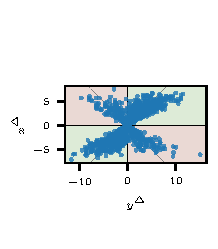
\includegraphics{plots/illustrative_examples/appendix_4q_dgp1}
        \caption{Constant \ac{atc} ratio.}
    \end{subfigure}\hspace{0.01\textwidth}
    \begin{subfigure}{0.24\textwidth}
        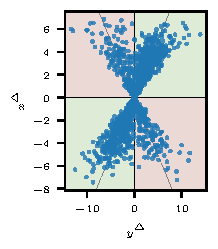
\includegraphics{plots/illustrative_examples/appendix_4q_dgp1_time}
        \caption{Time-varying \ac{atc} ratio}
    \end{subfigure}\hspace{0.01\textwidth}
    \begin{subfigure}{0.24\textwidth}
        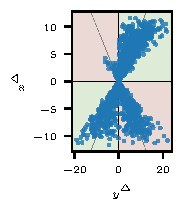
\includegraphics{plots/illustrative_examples/appendix_4q_dgp1_asym}
        \caption{Asymmetric \ac{atc} ratio}
    \end{subfigure}\hspace{0.01\textwidth}
    \begin{subfigure}{0.24\textwidth}
        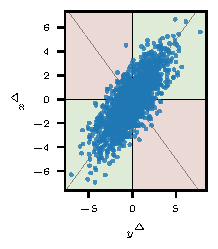
\includegraphics{plots/illustrative_examples/appendix_4q_dgp2}
        \caption{Second approach}
    \end{subfigure}
    \caption[Four-quadrant plots for sample realizations of the data generation schemes of Section~\ref{subsec:app-ATC-data-generation}.]{Four-quadrant plots for sample realizations of the data generation schemes of Section~\ref{subsec:app-ATC-data-generation}. Although the first and second plots differ over time, their difference is not discernible in the plots. The third data set's asymmetry is visible in the plot, but the decrease in the \ac{atc} near 0 is not visible. }
    \label{fig:appendix_dgps}
\end{figure}

\subsection{Simulation study on bootstrapping confidence intervals}\label{subsec:appendix-aatc-bootstrap}


We examine three methods for bootstrapping for computing confidence intervals for the \ac{atc} ratio: the intuitive percentile and the more sophisticated basic and \ac{bca} method.
In the \textit{percentile} approach, the confidence interval for the level $\alpha$ is built directly from the empirical distribution of the bootstrap estimators.
The \textit{basic} approach computes the confidence interval based on the non-bootstrap estimate using the bootstrapped quantile deviations~\citep{Davison1997}.
The \ac{bca} method modifies the quantiles of the empirical bootstrap distribution by a bias and an acceleration parameter~\citep{Efron1987}.
Typically, the percentile approach needs larger datasets and provides an easy and fast estimate, while the \ac{bca} is computationally expensive but requires smaller datasets for reasonable confidence intervals.
The basic approach balances these two objectives.
We compare the approaches in a small synthetic data study on their small-dataset behavior and computation time.

We vary the number of time steps $T$ to take typical time-series values, such as 30 for daily data in a month, 52 for weekly data, 168, 365, 720, and 1024.
The considered datasets are the first dataset with asymmetric dependence and the second dataset outlined in Appendix~\ref{subsec:app-ATC-data-generation}.
In the calculations, the \verb|scipy| package's implementation of bootstrap confidence intervals is used~\citep{Virtanen2020}.
The prescribed confidence level is 90 \%, and the number of bootstrap samples is $10,000$.
The share of confidence intervals covering the true values per method and $T$ are shown in Table~\ref{tab:atc_bootstrap}.
The true values of the accuracy are computed based on a dataset of size $10^8$, yielding 0.7501 and 0.7700 for the two datasets.
The computation times per method and dataset are shown in Figure~\ref{fig:atc_bootstrap_time}.
For the small sample sizes up to $T = 168$, only the \ac{bca} method keeps the confidence interval size and yields slightly wider confidence intervals.
The method's results are similar for the larger sample sizes.
The computation time for the \ac{bca} method is slightly larger than for the other methods, but all methods have a moderate computation time.
\Ac{bca} is the only method that maintains the confidence level for small datasets while increasing the computation time only moderately for larger datasets.
Therefore, we use the \ac{bca} method for confidence intervals in the applications in Section~\ref{sec:application}.


\begin{table}
    \centering
    \tiny
    \begin{subtable}{.48\textwidth}
       \centering
        \begin{tabular}{llll}
\toprule
 & percentile & basic & bca \\
\midrule
30 & 0.84 (0.249) & 0.86 (0.250) & 0.91 (nan) \\
52 & 0.89 (0.194) & 0.89 (0.193) & 0.89 (0.198) \\
168 & 0.91 (0.109) & 0.90 (0.109) & 0.90 (0.110) \\
365 & 0.90 (0.074) & 0.90 (0.074) & 0.90 (0.074) \\
720 & 0.90 (0.053) & 0.90 (0.053) & 0.90 (0.053) \\
1024 & 0.90 (0.044) & 0.90 (0.044) & 0.89 (0.044) \\
\bottomrule
\end{tabular}

        \caption{First dataset}
    \end{subtable}\hspace{0.02\textwidth}
    \begin{subtable}{.48\textwidth}
       \centering
       \begin{tabular}{llll}
\toprule
 & percentile & basic & BCa \\
\midrule
30 & 0.87 (0.243) & 0.88 (0.242) & 0.92 (0.249) \\
52 & 0.87 (0.188) & 0.89 (0.188) & 0.90 (0.192) \\
168 & 0.89 (0.106) & 0.90 (0.106) & 0.90 (0.107) \\
365 & 0.90 (0.072) & 0.90 (0.072) & 0.90 (0.072) \\
720 & 0.90 (0.052) & 0.90 (0.052) & 0.90 (0.052) \\
1024 & 0.89 (0.043) & 0.90 (0.043) & 0.90 (0.043) \\
\bottomrule
\end{tabular}

        \caption{Second dataset}
    \end{subtable}
    \caption[Proportion of bootstrapping confidence intervals covering the true value of \ac{atc} ratio per method and sample size $T$ in the bootstrap simulation study.]{Proportion of bootstrapping confidence intervals covering the true value of \ac{atc} ratio per method and sample size $T$. The average width of the confidence interval is listed in brackets.}
    \label{tab:atc_bootstrap}
\end{table}

\begin{figure}
    \centering
    \begin{subfigure}{0.48\textwidth}
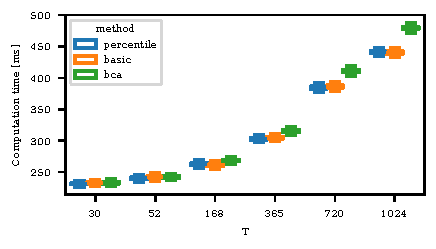
\includegraphics{plots/illustrative_examples/boxplot_comp_time_butterfly}
        \caption{First dataset}
    \end{subfigure}
    \begin{subfigure}{0.48\textwidth}
    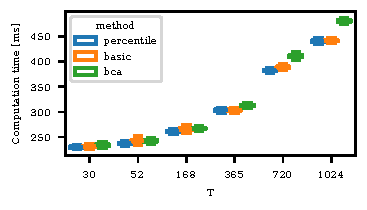
\includegraphics{plots/illustrative_examples/boxplot_comp_time_normal}
        \caption{Second dataset}
    \end{subfigure}
    \caption[Boxplot of the computation time for different bootstrapping methods and data set sizes.]{Boxplot of the computation time for different bootstrapping methods and data set sizes $T$. The computation time refers to bootstrapping one confidence interval based upon $10,000$ values. Each boxplot reflects $10,000$ samples. The \ac{bca} method takes slightly longer than the other two, but the difference is negligible.}
    \label{fig:atc_bootstrap_time}
\end{figure}


\subsection{Visualization of different bandwidth selectors in multivariate \ac{kde}}\label{subsec:appendix-kde}

We examine the resulting conditional \ac{atc} plots for the three well-known \ac{kde} bandwidth selectors, rule-of-thumb, cross-validation maximum likelihood, and cross-validation least squares using the \verb|statsmodels| Python package~\citep{Seabold2010} in Figure~\ref{fig:atc-cond-prob-bw}.
While the rule-of-thumb is based only on the covariance matrix, the other two numerically optimize the bandwidth with a hold-one-out least squares or likelihood objective function.
The dashed line shows the theoretical $P(\diffyrv \diffxrv > 0 | \diffxrv = \xcond)$.
The second method, cross-validation least squares, requires long computation times while yielding small or no bandwidth results, even for two relatively small datasets.
The rule-of-thumb and cross-validation maximum likelihood methods yield reasonable results at moderate computation times.

\begin{figure}
    \centering
    \begin{subfigure}{.48\textwidth}
        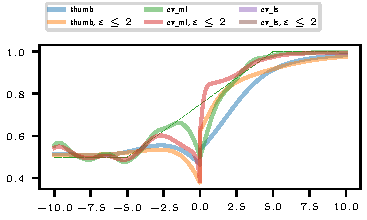
\includegraphics{plots/illustrative_examples/cond_prob_plot_bw_butterfly}
        \caption{First dataset with asymmetric dependence.}
    \end{subfigure}
    \begin{subfigure}{.48\textwidth}
        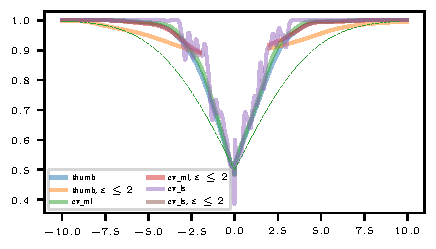
\includegraphics{plots/illustrative_examples/cond_prob_plot_bw_normal}
        \caption{Second dataset. }
    \end{subfigure}
    \caption[Conditional ATC plots for different bandwidth selection processes.]{Conditional \ac{atc} plot for different bandwidth selection processes. Cross-validation least squares takes a considerably larger computation time. It converges neither for the first nor the second data set with an exclusion area and yields a bandwidth too small for the second data set. The rule of thumb is the fastest method but tends to oversmooth. The cross-validation maximum likelihood method yields a more reasonable bandwidth with moderate computation time. $\varepsilon$ specifies an exclusion area $E = \{(x, y) \in \R^2: (-\varepsilon \leq x \leq \varepsilon)\}$ in $\diffx$-direction.}\label{fig:atc-cond-prob-bw}
\end{figure}




\subsection{Probabilistic ATC evaluation}\label{subsec:app-probabilistic-atc-evaluation}


Section~\ref{subsec:aatc-probabilistic} outlines the assessment of probabilistic \ac{atc} for nowcasts and forecasts and specifies the computation for predictions in terms of a \ac{cdf} and known true values.
Here, we outline the computation for quantile forecasts and yet unknown, probabilistic true values.

If forecasts or nowcasts are given as quantiles, $p_t$ can be determined by interpolations among the quantiles.
Let $q_p$ denote the quantiles for target time $t+l$ for even-spaced probabilities $p \in \{1/\pmax, \dots, (p-1) / \pmax\}$ ($\pmax \in \N \setminus \{1, 2\}$) and $y_t$ the true value at time $t$.
The quantiles $q_p$ generally differ for each time step, but we omit an index here for ease of notation.
The probability $\pc_t$ of a \textit{negative} change is between $p^{\star}$ and $p^{\star} + 1/\pmax$ for
\begin{equation*}
    p^{\star} = \max \{p \in \{1/\pmax, \dots, (\pmax-1) / \pmax\}: q_p \leq y_t\} , \quad \text{if}\ q_{1/\pmax} \leq y_t \leq q_{1 - 1/\pmax}.
\end{equation*}
Quantiles do not determine the location within the interval $[p^{\star}, p^{\star} + 1/\pmax]$.
Under the assumption of a uniform distribution within the quantile interval, the probability of a negative change is
\begin{equation*}
    \pc_t = \frac{y_t - q_{p^\star}}{\pmax (q_{p^{\star} + 1} - q_{p^{\star}})} + p^{\star}.
\end{equation*}
The approach does not yet assign probabilities for $y_t$ smaller than the smallest quantile $q_{1/p}$ or greater than the largest quantile.
As a simple extension, we assume that the probability mass is uniformly distributed on an interval of the same length as the nearest interval specified by the quantiles.
This yields
\begin{equation*}
\pc_t = \begin{cases}
    \max \{\frac{1}{\pmax} - \frac{q_{p^\star} - y_t}{\pmax (q_{p2/\pmax} - q_{1/\pmax})}, 0\} &, \text{if } y_t < q_{1/p}, \\
    \min \{\frac{1}{\pmax} - \frac{y_t - q_{(\pmax-1)/\pmax}}{\pmax (q_{(\pmax-1)/\pmax} - q_{(\pmax-2)/\pmax})}, 1\} &, \text{if } y_t > q_{1 - 1/p}, \\
    \frac{y_t - q_{p^\star}}{\pmax (q_{p^{\star} + 1} - q_{p^{\star}})} + p^{\star} &, \text{otherwise.}
\end{cases}
\end{equation*}
The probability of positive change is $p_t = 1 - \pc_t$.

If the true value is given as a distribution because it is still unknown, the probabilities $p_t$ can be computed by integration.
Let for two nowcasts the distributions be given by \acp{pdf} $f_{t+l|t+l}$ and $f_{t|t+l}$ with \acp{cdf}  $F_{t+l|t+l}$ and $F_{t|t+l}$.
Then, the probability of a negative change can be computed by
\begin{align}
    \pc_t
        &= \int_{\begin{subarray}{l}x_1, x_2 \in \R: \\ x_2 < x_1\end{subarray}} f_{t|t+l} (x_1) f_{t+l|t+l} (x_2)  \ \textrm{d} \: (x_1, x_2) \nonumber\\
        &= \int_{x_1 \in \R} \int_{-\infty}^{x_1} f_{t|t+l} (x_1) f_{t+l|t+l} (x_2)  \ \textrm{d} \: x_2 \ \textrm{d} \: x_1 \nonumber\\
        &= \int_{x_1 \in \R} f_{t|t+l} (x_1) F_{t+l|t+l} (x_1)  \ \textrm{d} \: x_2 \ \textrm{d} \: x_1 \label{eq:atc-probabilistic-pdf}.
\end{align}
Thereby, the distributions are assumed to be independent.
If the nowcasts have the form of a multivariate distribution, including the dependence of the two \acp{pdf}, $f_{t+l|t+l} (x_2)$ has to be replaced by the \ac{pdf} conditional on $x_1$.
As a Monte Carlo approximation of Equation~\eqref{eq:atc-probabilistic-pdf}, the probability can also be calculated by sampling from $f_{t+l|t+l}$ and $f_{t|t+l}$ and calculating the fraction of negative changes.
For forecasts, the indexes have to be shifted.
If no \acp{pdf} are available, they can be estimated from the \ac{cdf} or quantiles, or the \ac{cdf} or quantiles can be used to generate samples for the Monte Carlo approximation.
This approach is applied in Section~\ref{sec:application-covid}, as the true values are published with a delay of more than 80 days, and the nowcasts are given as quantiles.


\section{Additional results for Section~\ref{sec:application-covid}}\label{sec:appendix-application-covid}

\begin{figure}
    \centering
    \begin{subfigure}[t]{0.48\textwidth}
    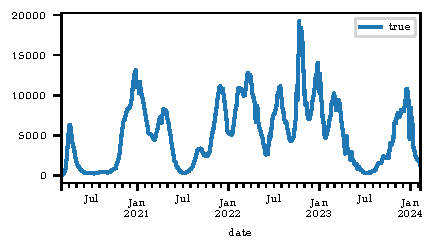
\includegraphics{plots/covid_nowcast/00_true_data}
    \caption{Realisations.}
    \label{fig:app-covid-true}
    \end{subfigure}\hfill
    \begin{subfigure}[t]{0.48\textwidth}
    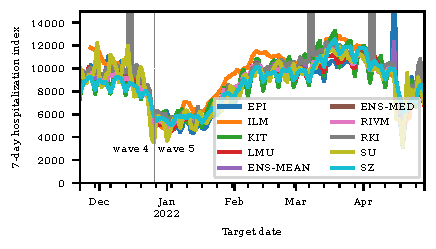
\includegraphics{plots/covid_nowcast/00_nowcast_data}
    \caption{Same-day nowcasts.}
    \label{fig:app-covid-nowcast}
        \end{subfigure}
    \caption[True and nowcast data of the seven-day-hospitalization in Germany from November 22, 2021, to April 29, 2022.]{True and nowcast data of the seven-day-hospitalization in Germany from November 22, 2021, to April 29, 2022 \citep{ChairOfEconometricsAndStatisticsAtKarlsruheInstituteOfTechnology2024}.
    The outliers in the RKI model of values above $10^8$ are removed before the following analysis.}
    \label{fig:app-covid-true-nowcast}
\end{figure}

\begin{table}
    \centering
    \begin{tabular}{l l}
        \toprule
        Abbreviation & Nowcasting hub key \\
        \midrule
        EPI & Epiforecasts-independent \\
        ILM & ILM-prop \\
        KIT & KIT-simple\_nowcast \\
        LMU & LMU\_StaBLab-GAM\_nowcast \\
        RIVM & RIVM-KEW \\
        RKI & RKI-weekly\_report \\
        SU & SU-hier\_bayes \\
        SZ & SZ-hosp\_nowcast\\
        ENS-MEAN & NowcastHub-MeanEnsemble\\
        ENS-MED & NowcastHub-MedianEnsemble\\
        \bottomrule
    \end{tabular}
    \caption[Matching the abbreviation to the key in the Covid nowcasting hub.]{Matching the abbreviation to the key in the Covid nowcasting hub.
    Information on the models and references is listed in \citet[][Table 1]{Wolffram2023}.}
    \label{tab:app-covid-models}
\end{table}


\begin{table}
    \centering
    \tiny
    \begin{tabularx}{\textwidth}{Xlllllllll}
\toprule
 & (1), l=1 & $\sigma_{x^{\Delta, 1}}$ & $q_{0.1} (x^{\Delta, 1})$ & (1), l=7 & $\sigma_{x^{\Delta, 7}}$ & $q_{0.1} (x^{\Delta, 7})$ & (1), l=14 & $\sigma_{x^{\Delta, 14}}$ & $q_{0.1} (x^{\Delta, 14})$ \\
\midrule
EPI & 86 & 520 & 44 & 83 & 1411 & 78 & 80 & 1976 & 144 \\
ILM & 86 & 281 & 26 & 81 & 1457 & 102 & 82 & 2356 & 140 \\
KIT & 84 & 354 & 50 & 89 & 1306 & 171 & 83 & 1964 & 265 \\
LMU & 65 & 285 & 26 & 84 & 1180 & 124 & 78 & 1946 & 167 \\
ENS-MEAN & 85 & 267 & 23 & 86 & 1213 & 98 & 83 & 1955 & 235 \\
ENS-MED & 88 & 259 & 23 & 88 & 1206 & 101 & 81 & 1955 & 186 \\
RIVM & 77 & 241 & 32 & 81 & 1264 & 123 & 77 & 2034 & 190 \\
RKI & 99 & 362 & 34 & 106 & 1194 & 145 & 99 & 1832 & 325 \\
SU & 91 & 376 & 47 & 85 & 1390 & 180 & 80 & 2126 & 263 \\
SZ & 92 & 201 & 26 & 89 & 1154 & 184 & 87 & 1889 & 241 \\
True & 75 & 262 & 27 & 66 & 1237 & 126 & 73 & 2193 & 284 \\
\bottomrule
\end{tabularx}

    \caption[Marginal analysis of the Covid nowcast and true changes for the horizons one, seven, and 14 days.]{Marginal analysis of the Covid nowcast and true changes for the horizons one, seven, and 14 days.
    The column (1), $l=l$ shows the number of values greater than zero for horizon $l$, $\sigma_{x^{\Delta, l}}$ the standard deviation, and $q_{0.1} (x^{\Delta, l})$ the 10\% quantile of the changes' absolute values.}
    \label{tab:app-covid-marginals}
\end{table}

\begin{table}
    \centering
    \tiny
    \begin{subtable}[t]{\textwidth}
        \begin{tabular}{l p{0.11\textwidth} p{0.11\textwidth} p{0.11\textwidth} p{0.11\textwidth} p{0.11\textwidth} p{0.11\textwidth}}
\toprule
 & $\mu^{1}$ & $\mu^{+, 1}$ & $\mu^{-, 1}$ & $\mu^{1}_{q_{0.1}}$ & $\mu^{+, 1}_{q_{0.1}}$ & $\mu^{-, 1}_{q_{0.1}}$ \\
\midrule
EPI & {0.68\newline(0.62, 0.74)} & {0.64\newline(0.55, 0.72)} & {0.73\newline(0.63, 0.81)} & {0.69\newline(0.63, 0.75)} & {0.64\newline(0.56, 0.73)} & {0.75\newline(0.65, 0.82)} \\
ILM & {0.73\newline(0.67, 0.79)} & {0.67\newline(0.58, 0.76)} & {0.82\newline(0.73, 0.89)} & {0.74\newline(0.68, 0.79)} & {0.68\newline(0.60, 0.76)} & {0.82\newline(0.72, 0.89)} \\
KIT & {0.62\newline(0.55, 0.68)} & {0.58\newline(0.49, 0.67)} & {0.65\newline(0.56, 0.75)} & {0.62\newline(0.56, 0.69)} & {0.59\newline(0.51, 0.67)} & {0.66\newline(0.57, 0.74)} \\
LMU & {0.66\newline(0.60, 0.72)} & {0.66\newline(0.57, 0.75)} & {0.66\newline(0.57, 0.73)} & {0.66\newline(0.59, 0.72)} & {0.66\newline(0.55, 0.75)} & {0.66\newline(0.57, 0.73)} \\
ENS-MEAN & {0.81\newline(0.75, 0.85)} & {0.76\newline(0.68, 0.84)} & {0.88\newline(0.81, 0.93)} & {0.81\newline(0.75, 0.86)} & {0.76\newline(0.68, 0.83)} & {0.88\newline(0.81, 0.94)} \\
ENS-MED & {0.75\newline(0.68, 0.80)} & {0.69\newline(0.60, 0.77)} & {0.81\newline(0.73, 0.89)} & {0.75\newline(0.69, 0.80)} & {0.69\newline(0.61, 0.77)} & {0.83\newline(0.74, 0.90)} \\
RIVM & {0.77\newline(0.72, 0.82)} & {0.75\newline(0.66, 0.83)} & {0.79\newline(0.71, 0.85)} & {0.78\newline(0.72, 0.83)} & {0.75\newline(0.66, 0.83)} & {0.81\newline(0.73, 0.87)} \\
RKI & {0.74\newline(0.68, 0.80)} & {0.67\newline(0.59, 0.75)} & {0.88\newline(0.79, 0.93)} & {0.74\newline(0.67, 0.79)} & {0.66\newline(0.58, 0.73)} & {0.87\newline(0.78, 0.93)} \\
SU & {0.71\newline(0.65, 0.77)} & {0.66\newline(0.57, 0.74)} & {0.78\newline(0.69, 0.85)} & {0.72\newline(0.66, 0.78)} & {0.67\newline(0.58, 0.75)} & {0.79\newline(0.70, 0.87)} \\
SZ & {0.74\newline(0.69, 0.80)} & {0.68\newline(0.60, 0.76)} & {0.82\newline(0.73, 0.88)} & {0.74\newline(0.69, 0.80)} & {0.68\newline(0.60, 0.76)} & {0.82\newline(0.73, 0.88)} \\
\bottomrule
\end{tabular}

    \caption{1 day.}
    \end{subtable}
    \begin{subtable}[t]{\textwidth}
        \begin{tabular}{l p{0.11\textwidth} p{0.11\textwidth} p{0.11\textwidth} p{0.11\textwidth} p{0.11\textwidth} p{0.11\textwidth}}
\toprule
 & $\mu^{14}$ & $\mu^{+, 14}$ & $\mu^{-, 14}$ & $\mu^{14}_{q_{0.1}}$ & $\mu^{+, 14}_{q_{0.1}}$ & $\mu^{-, 14}_{q_{0.1}}$ \\
\midrule
EPI & {0.83\newline(0.77, 0.87)} & {0.79\newline(0.70, 0.85)} & {0.87\newline(0.80, 0.92)} & {0.85\newline(0.80, 0.90)} & {0.81\newline(0.73, 0.87)} & {0.90\newline(0.83, 0.95)} \\
ILM & {0.86\newline(0.81, 0.90)} & {0.78\newline(0.70, 0.85)} & {0.96\newline(0.90, 0.99)} & {0.87\newline(0.82, 0.91)} & {0.80\newline(0.71, 0.86)} & {0.96\newline(0.90, 0.99)} \\
KIT & {0.81\newline(0.75, 0.86)} & {0.76\newline(0.67, 0.83)} & {0.87\newline(0.79, 0.92)} & {0.82\newline(0.76, 0.86)} & {0.76\newline(0.68, 0.84)} & {0.88\newline(0.81, 0.93)} \\
LMU & {0.88\newline(0.83, 0.92)} & {0.85\newline(0.77, 0.91)} & {0.91\newline(0.85, 0.95)} & {0.89\newline(0.85, 0.93)} & {0.87\newline(0.79, 0.92)} & {0.91\newline(0.85, 0.95)} \\
ENS-MEAN & {0.83\newline(0.77, 0.87)} & {0.77\newline(0.69, 0.84)} & {0.89\newline(0.83, 0.95)} & {0.84\newline(0.78, 0.88)} & {0.78\newline(0.70, 0.85)} & {0.91\newline(0.84, 0.95)} \\
ENS-MED & {0.84\newline(0.79, 0.89)} & {0.79\newline(0.70, 0.85)} & {0.90\newline(0.83, 0.95)} & {0.85\newline(0.80, 0.90)} & {0.80\newline(0.72, 0.86)} & {0.91\newline(0.84, 0.96)} \\
RIVM & {0.85\newline(0.80, 0.89)} & {0.82\newline(0.74, 0.88)} & {0.88\newline(0.80, 0.93)} & {0.85\newline(0.80, 0.90)} & {0.83\newline(0.75, 0.89)} & {0.88\newline(0.80, 0.93)} \\
RKI & {0.81\newline(0.75, 0.86)} & {0.71\newline(0.63, 0.77)} & {0.98\newline(0.93, 1.00)} & {0.81\newline(0.75, 0.86)} & {0.71\newline(0.63, 0.78)} & {1.00\newline(nan, nan)} \\
SU & {0.88\newline(0.83, 0.92)} & {0.84\newline(0.76, 0.90)} & {0.92\newline(0.86, 0.96)} & {0.89\newline(0.84, 0.93)} & {0.85\newline(0.77, 0.91)} & {0.94\newline(0.87, 0.97)} \\
SZ & {0.82\newline(0.77, 0.87)} & {0.76\newline(0.68, 0.83)} & {0.90\newline(0.83, 0.94)} & {0.83\newline(0.78, 0.88)} & {0.78\newline(0.69, 0.85)} & {0.90\newline(0.83, 0.94)} \\
\bottomrule
\end{tabular}

        \caption{14 days.}
    \end{subtable}
    \caption[ATC ratios for the models without and with exclusion areas for the horizon one and 14 days in Covid nowcasting.]{\Ac{atc} ratio $\acc$, positive \ac{atc} ratio $\accp$, and negative \ac{atc} ratio $\accm$ for the models without and with exclusion areas for the horizon one and 14 days in Covid nowcasting. The exclusion areas are rectangles centered on the zero points with a width and height to exclude the 10\%-quantile of the absolute values of nowcast or true values. }
    \label{tab:app-covid-atc-ratios-lag-1-14}
\end{table}



\begin{figure}
\centering
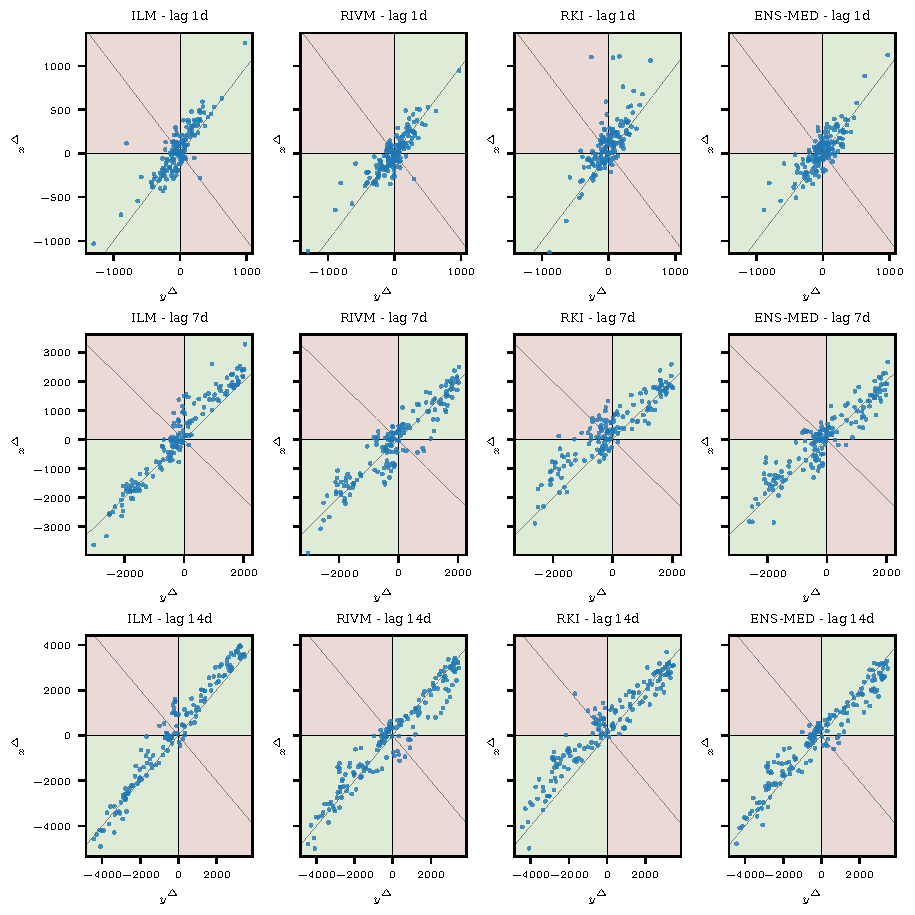
\includegraphics{plots/covid_nowcast/30_4q_plots}
\caption[Four-quadrant plots for the Covid nowcast models ILM, RIVM, RKI, and ENS-MEAN and the horizons of one, seven, and 14 days.]{Four-quadrant plots for the Covid nowcast models ILM, RIVM, RKI, and ENS-MEAN and the horizons of one, seven, and 14 days. The spread in both directions increases with the horizon. }
\label{fig:app-covid-4q}
\end{figure}


\begin{figure}
    \centering
%    \includegraphics{}
    \begin{subfigure}[t]{.48\textwidth}
    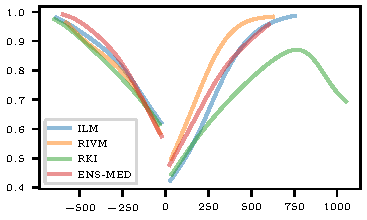
\includegraphics{plots/covid_nowcast/40_cond_prob_lag_1}
    \caption{Conditional \ac{atc} plot for horizon 1.}\label{fig:app-covid-cond-prob-1}
    \end{subfigure}\hfill
    \begin{subfigure}[t]{.48\textwidth}
    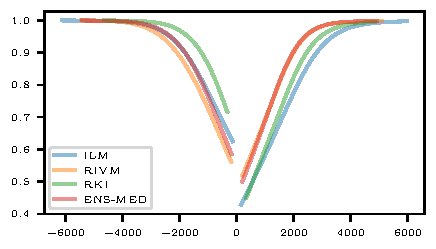
\includegraphics{plots/covid_nowcast/40_cond_prob_lag_14}
    \caption{Conditional \ac{atc} plot for horizon 1.}\label{fig:app-covid-cond-prob-14}
    \end{subfigure}
    \begin{subfigure}[t]{.48\textwidth}
    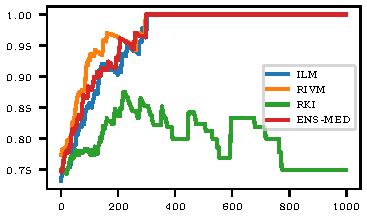
\includegraphics{plots/covid_nowcast/40_acc_eps_lag_1}
    \caption{\Ac{atc} ratio over exclusion area size in $\diffx$ for horizon 1.}\label{fig:app-covid-atc-ratio-1}
    \end{subfigure}\hfill
    \begin{subfigure}[t]{.48\textwidth}
    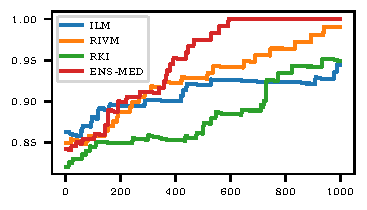
\includegraphics{plots/covid_nowcast/40_acc_eps_lag_14}
    \caption{\ac{atc} ratio over exclusion area size in $\diffx$ for horizon 1.}\label{fig:app-covid-atc-ratio-14}
    \end{subfigure}
    \caption[Conditional ATC plot and ATC ratio over exclusion area in Covid nowcasting.]{Conditional \ac{atc} plot and \ac{atc} ratio over exclusion area for the Covid nowcasts of the seven-day hospitalization rate ILM, RKI, RIVM, and ENS-MED for the horizon seven days.}
    \label{fig:app-covid-cond-prob-atc-ratio-1-14}
\end{figure}


\begin{figure}
    \centering
    \begin{subfigure}[t]{.48\textwidth}
        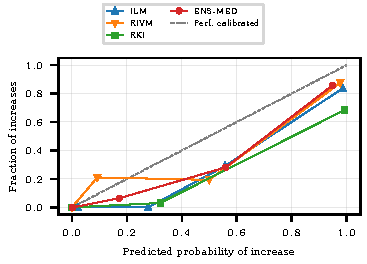
\includegraphics{plots/covid_nowcast/60_reliability_diagram_lag_7}
        \caption{Reliability diagram for horizon seven days.} \label{fig:app-covid-reliability-7}
    \end{subfigure}\hfill
    \begin{subfigure}[t]{.48\textwidth}
        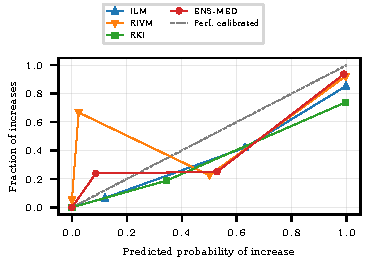
\includegraphics{plots/covid_nowcast/60_reliability_diagram_lag_14}
        \caption{Reliability diagram for horizon 14 days.} \label{fig:app-covid-reliability-14}
    \end{subfigure}
    \begin{subfigure}{\textwidth}
        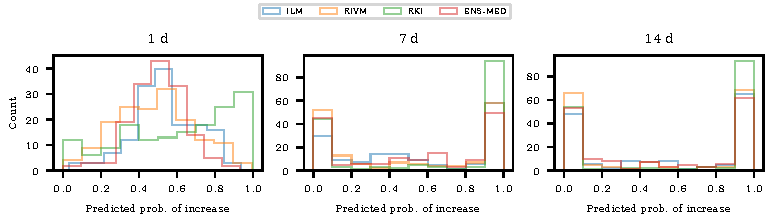
\includegraphics{plots/covid_nowcast/70_prob_hist}
        \caption{Count histogram of the predicted probabilities for the horizon one, seven, and 14 days.} \label{fig:app-covid-prob-hist}
    \end{subfigure}
    \caption[Reliability diagrams for Covid nowcasting models and the horizon seven and 14 days.]{The reliability diagram for the Covid nowcasting models ILM, RIVM, RKI, and ENS-MED for the horizon seven and 14 days.
    Additionally, the count of predicted probabilities for the horizons is shown.
        The reliability diagram bins are chosen according to the empirical quantiles of the predicted probabilities.
    As the models issue small or large probabilities of increase for the higher horizons, little information on the accuracy of moderate probability predictions is available.}
    \label{fig:app-covid-rel}
\end{figure}
%TC:endignore



\end{document} 
